%%%%%%%%%%%%%%%%%%%%%%%%%%%%%%%%%%%%%%%%%%%%%%%%%%%%%%%%%%%%%%%%%%%%%%%%%%%%%%%
% Memorial para concurso público de Pesquisador Adjunto I em Sismologia.
%
% Formatação inspirada em:
% * https://github.com/leouieda/memorial2023/tree/main
%%%%%%%%%%%%%%%%%%%%%%%%%%%%%%%%%%%%%%%%%%%%%%%%%%%%%%%%%%%%%%%%%%%%%%%%%%%%%%%

%%%%%%%%%%%%%%%%%%%%%%%%%%%%%%%%%%%%%%%%%%%%%%%%%%%%%%%%%%%%%%%%%%%%%%%%%%%%%%%
% Set a class and import packages
\documentclass[10pt,a4paper,oneside]{book}

% Variables
\newcommand{\Year}{2024}
\newcommand{\Author}{Diogo Luiz de Oliveira Coelho}
\newcommand{\Title}{Memorial de \Author{} para concurso público - Pesquisador Adjunto I em Sismologia - ON/MCTI}
\newcommand{\Email}{diogoloc@on.br}
\newcommand{\EmailPersonal}{locdiogo@gmail.com}
\newcommand{\ORCID}{0000-0001-5426-0455}
\newcommand{\ResearchGate}{https://www.researchgate.net/profile/Diogo-De-Oliveira-Coelho}
\newcommand{\Lattes}{4330106475199471}

% Import packages
\usepackage[utf8]{inputenc}
\usepackage[T1]{fontenc}
\usepackage[brazil]{babel}
\usepackage{geometry}
\usepackage{graphicx}
\usepackage{amssymb}
\usepackage{amsmath}
\usepackage{mathpazo}
\usepackage{hyperref}
% create fancy headers
\usepackage{fancyhdr}
% commands for managing dates and its formats
\usepackage{datetime2}
% improved urls with proper hyphenation
\usepackage{xurl}
% Control over enumerate and itemize
\usepackage{enumitem}
% Tweak the look of captions
\usepackage{caption}
% To control the style of section titles
\usepackage{titlesec}
% Add the bibliography to the table of contents
\usepackage[nottoc,chapter]{tocbibind}
\usepackage[round,authoryear,sort]{natbib}
% show dois as links on references
\usepackage{doi}
% Icon and fonts (requires using xelatex or luatex)
\usepackage{fontawesome5}
\usepackage{academicons}
\usepackage{fontspec}
\usepackage[mono]{notomath}
% To make everything neater
\usepackage{microtype}
% To make fancy text boxes
\usepackage{xcolor}
\usepackage[framemethod=default]{mdframed}
% For fancy and multipage tables
\usepackage{tabularx}
\usepackage{ltablex}
% To define custom environments
\usepackage{environ}
\usepackage{setspace}
% Reference sections by name
\usepackage{nameref}
% Better handling of footnotes inside summary boxes
\usepackage{footmisc}

%to rotate the page
\usepackage{pdflscape}

%To plot piechart
\usepackage{bera}
\usepackage{pstricks-add}
\usepackage{pgf-pie}


%%%%%%%%%%%%%%%%%%%%%%%%%%%%%%%%%%%%%%%%%%%%%%%%%%%%%%%%%%%%%%%%%%%%%%%%%%%%%%%

%%%%%%%%%%%%%%%%%%%%%%%%%%%%%%%%%%%%%%%%%%%%%%%%%%%%%%%%%%%%%%%%%%%%%%%%%%%%%%%
% Configuration of the document

\geometry{%
  left=30mm,
  right=30mm,
  top=20mm,
  bottom=15mm,
  headsep=5mm,
  headheight=5mm,
  footskip=10mm,
  includehead=true,
  includefoot=true
}

% Increase the line spacing
\SetSinglespace{1.2}
\onehalfspacing

% Remove spacing between enumerate/itemize items
\setlist{nosep}

% Padding between the first figure and the chapter title
\newcommand{\HeroFigPad}{\vspace{-1cm}}

% Padding before the software logo figures
\newcommand{\SoftwareFigPad}{\vspace{-0.3cm}}

% Add a link to a DOI
\newcommand{\DOI}[1]{\url{https://doi.org/#1}}

% Add a link to a GitHub repository
\newcommand{\GitHub}[1]{\faGithub{} Código: \url{https://github.com/#1}}

% Add a link to a YouTube video
\newcommand{\YouTube}[1]{\faYoutube{} Vídeo: \url{https://youtu.be/#1}}

% Add a link to a supplementary data
\newcommand{\Data}[1]{\faChartBar{} Dados: \url{https://doi.org/#1}}

% Add a link to a preprint
\newcommand{\Preprint}[1]{\faLockOpen{} Preprint: \url{https://doi.org/#1}}

% Make a Unicode bullet symbol
\newcommand{\Bullet}{•\enspace}

% Define custom colors
\definecolor{lu_gray}{gray}{0.98}
\definecolor{lu_darkgray}{gray}{0.3}
\definecolor{lu_blue}{RGB}{32, 96, 194}
\definecolor{lu_lightblue}{RGB}{238, 245, 250}
\definecolor{lu_yellow}{RGB}{255, 193, 7}
\definecolor{lu_lightyellow}{RGB}{255, 249, 230}

% Customize how Chapter headings are displayed
\titleformat{\chapter}[display]{\normalfont}{\large Capítulo \thechapter}{0pt}{\huge}[\titlerule]
\titlespacing*{\chapter}{0pt}{-40pt}{40pt}

% Set the spacing between bibliography entries (requires natbib)
\setlength{\bibsep}{0pt}

% Configure captions
\captionsetup{labelfont=bf,font={small,color=lu_darkgray},skip=0pt}

% Define a fancy text box
\mdfdefinestyle{summarybox}{%
  leftline=true,
  rightline=false,
  topline=false,
  bottomline=false,
  linewidth=4pt,
  linecolor=lu_blue,
  frametitlefont=\bfseries\color{black}\small,
  frametitlebackgroundcolor=lu_lightblue,
  frametitleaboveskip=7pt,
  frametitlebelowskip=7pt,
  frametitlerule=true,
  frametitlerulewidth=1pt,
  backgroundcolor=lu_gray,
  innertopmargin=7pt,
  innerbottommargin=10pt,
  innerleftmargin=15pt,
  innerrightmargin=15pt,
  skipbelow=5pt,
  skipabove=0pt,
}
\newmdenv[style=summarybox]{summarybox}
\mdfdefinestyle{subsummarybox}{%
  leftline=true,
  rightline=false,
  topline=false,
  bottomline=false,
  linewidth=4pt,
  linecolor=lu_yellow,
  frametitlefont=\bfseries\color{black}\small,
  frametitlebackgroundcolor=lu_lightyellow,
  frametitleaboveskip=7pt,
  frametitlebelowskip=7pt,
  frametitlerule=true,
  frametitlerulewidth=1pt,
  backgroundcolor=lu_gray,
  innertopmargin=7pt,
  innerbottommargin=10pt,
  innerleftmargin=15pt,
  innerrightmargin=15pt,
  skipbelow=5pt,
  skipabove=0pt,
}
\newmdenv[style=subsummarybox]{subsummarybox}

% Define something like an fa-ul and a date list
\NewEnviron{fa-ul}{%
  \vspace{-0.4cm}
  \small
  \renewcommand{\arraystretch}{1.25}
  \begin{tabularx}{\linewidth}{@{}p{0.05\linewidth}@{}@{}p{0.95\linewidth}@{}}
    \BODY
  \end{tabularx}%
}
\NewEnviron{datelist}{%
  \vspace{-0.4cm}
  \small
  \renewcommand{\arraystretch}{1.25}
  \begin{tabularx}{\linewidth}{@{}p{0.15\linewidth}@{}@{}p{0.85\linewidth}@{}}
    \BODY
  \end{tabularx}%
}
\NewEnviron{paperlist}{%
  \vspace{-0.4cm}
  \small
  \renewcommand{\arraystretch}{1.25}
  \begin{tabularx}{\linewidth}{@{}p{0.08\linewidth}@{}@{}p{0.92\linewidth}@{}}
    \BODY
  \end{tabularx}%
}
\NewEnviron{courselist}{%
  \vspace{-0.4cm}
  \small
  \renewcommand{\arraystretch}{1.25}
  \begin{tabularx}{\linewidth}{@{}p{0.15\linewidth}@{}@{}p{0.85\linewidth}@{}}
    \BODY
  \end{tabularx}
}

% Define a fancy enumerate that has a title
\NewEnviron{fancyenum}[2]{%
  \vspace{0.25cm}
  \noindent#1\quad\textbf{#2}:
  \vspace{0.25cm}
  \begin{enumerate}
    \BODY
  \end{enumerate}
}

% Configure hyperref and add PDF metadata
\hypersetup{
    colorlinks,
    allcolors=lu_blue,
    pdftitle={\Title},
    pdfauthor={\Author},
    pdftex,
    breaklinks=true,
}

% make urls use the same font as every other text
\urlstyle{same}

% Prevent footnotes from being broken into multiple pages
\interfootnotelinepenalty=10000

% Configure headers and footers
\fancyhf{}
\lhead{\fontsize{9pt}{0}\selectfont\itshape \nouppercase\leftmark}
\chead{}
\rhead{\fontsize{9pt}{0}\selectfont \thepage}
\cfoot{}
\renewcommand{\headrulewidth}{0.3pt}
%%%%%%%%%%%%%%%%%%%%%%%%%%%%%%%%%%%%%%%%%%%%%%%%%%%%%%%%%%%%%%%%%%%%%%%%%%%%%%%

%%%%%%%%%%%%%%%%%%%%%%%%%%%%%%%%%%%%%%%%%%%%%%%%%%%%%%%%%%%%%%%%%%%%%%%%%%%%%%%
\begin{document}

\pagestyle{plain}
\frontmatter

\begin{titlepage}
  \begin{center}
    
\includegraphics[height=2cm]{images/logo_seismo.png}
    \vspace{1cm}

    CONCURSO PÚBLICO
    
    PESQUISADOR ADJUNTO I EM SISMOLOGIA
    
    OBSERVATÓRIO NACIONAL

    \vspace{5cm}

    \textbf{\LARGE Memorial}
    \vspace{1cm}

    \textbf{\LARGE \MakeUppercase{\Author{}}}
    \vspace{5cm}

    {\small
	Apresentado para concurso público de provas e títulos para cargo de

	Pesquisador Adjunto I em Sismologia à Coordenação de Geofísica do

	Observatório Nacional.
      \vspace{1cm}

	EDITAL Nº 1, DE 9 DE OUTUBRO DE 2023
    }
    \vfill

    \Year{}
  \end{center}
\end{titlepage}

%==============================================================================
\chapter*{Resumo}

Ao longo da minha trajetória acadêmica, obtive sucesso ao concluir o bacharelado em \href{https://geologia.ufes.br/}{Geologia} pela Universidade Federal do Espírito Santo, o mestrado em \href{https://www.gov.br/observatorio/pt-br/assuntos/programas-academicos/pos-graduacao-em-geofisica/pos-graduacao-em-geofisica}{Geofísica} pelo Observatório Nacional e o doutorado em \href{https://posgraduacao.ufrn.br/325}{Geodinâmica e Geofísica} pela Universidade Federal do Rio Grande do Norte. Durante minha formação acadêmica, tive a oportunidade de passar por três instituições de ensino superior ligadas ao Ministério da Educação (MEC), uma unidade de pesquisa vinculada ao Ministério da Ciência, Tecnologia e Inovações (MCTI), além de realizar estágio de nível superior na Petrobras, uma empresa estatal do setor de energia. Nessa caminhada acadêmica, tive a oportunidade enriquecedora de vivenciar de perto instituições públicas em quatro estados distintos do país. Essa diversidade geográfica proporcionou-me um aprendizado valioso e o aprimoramento da minha atuação na academia. Desde minha entrada no Observatório Nacional, ministrei a disciplina de \href{https://www.gov.br/observatorio/pt-br/assuntos/programas-academicos/pos-graduacao-em-geofisica/grade-curricular}{Introdução à Sismologia} em nível de pós-graduação, cursos de curta duração para graduandos em outras instituições e orientei alunos de iniciação científica. No âmbito da divulgação e popularização da ciência, redigi diversas notas técnicas tanto para a instituição quanto para veículos de imprensa. Além disso, participei de mais de 35 eventos relacionados a popularização e divulgação da ciência, dentre feiras de tecnologia, entrevistas para diversos canais da imprensa, podcast, revisão de textos e notas técnicas explorando temas variados da sismologia, incluindo sua relação com desastres naturais, bem como curiosidades gerais da população sobre a atuação de um pesquisador em geofísica. Desde o mestrado, tenho atuado na área de Sismologia e Tectônica da Crosta. Já no doutorado iniciei, de forma sistemática, o processo de desenvolvimento de diversos códigos em \href{https://www.python.org/}{python} para a sismologia, incluindo \href{https://github.com/dIOGOLOC/codes_escritos/tree/master/mantle_transition_zone_migration_obspy_Pds}{Receiver Migration}, \href{https://zooxantelapy.readthedocs.io/en/latest/}{Zooxantelapy} e \href{https://github.com/dIOGOLOC/marefone/wiki}{Marefone}. O primeiro pacote está relacionado a estruturação do manto terrestre e os dois últimos à dados oriundos de redes subaquáticas, às quais iniciei o tratamento e processamento de dados em 2020. Este memorial apresenta de forma resumida minha formação e atuação acadêmica, incluindo algumas considerações sobre os fatores que influenciaram na minha trajetória e os principais ensinamentos adquiridos ao longo dessa jornada que me ajudaram fazer pequenos ajustes na rota até aqui.

\begin{landscape}
% Conteúdo da página em modo paisagem
\begin{figure}[tb]
  \begin{center}
    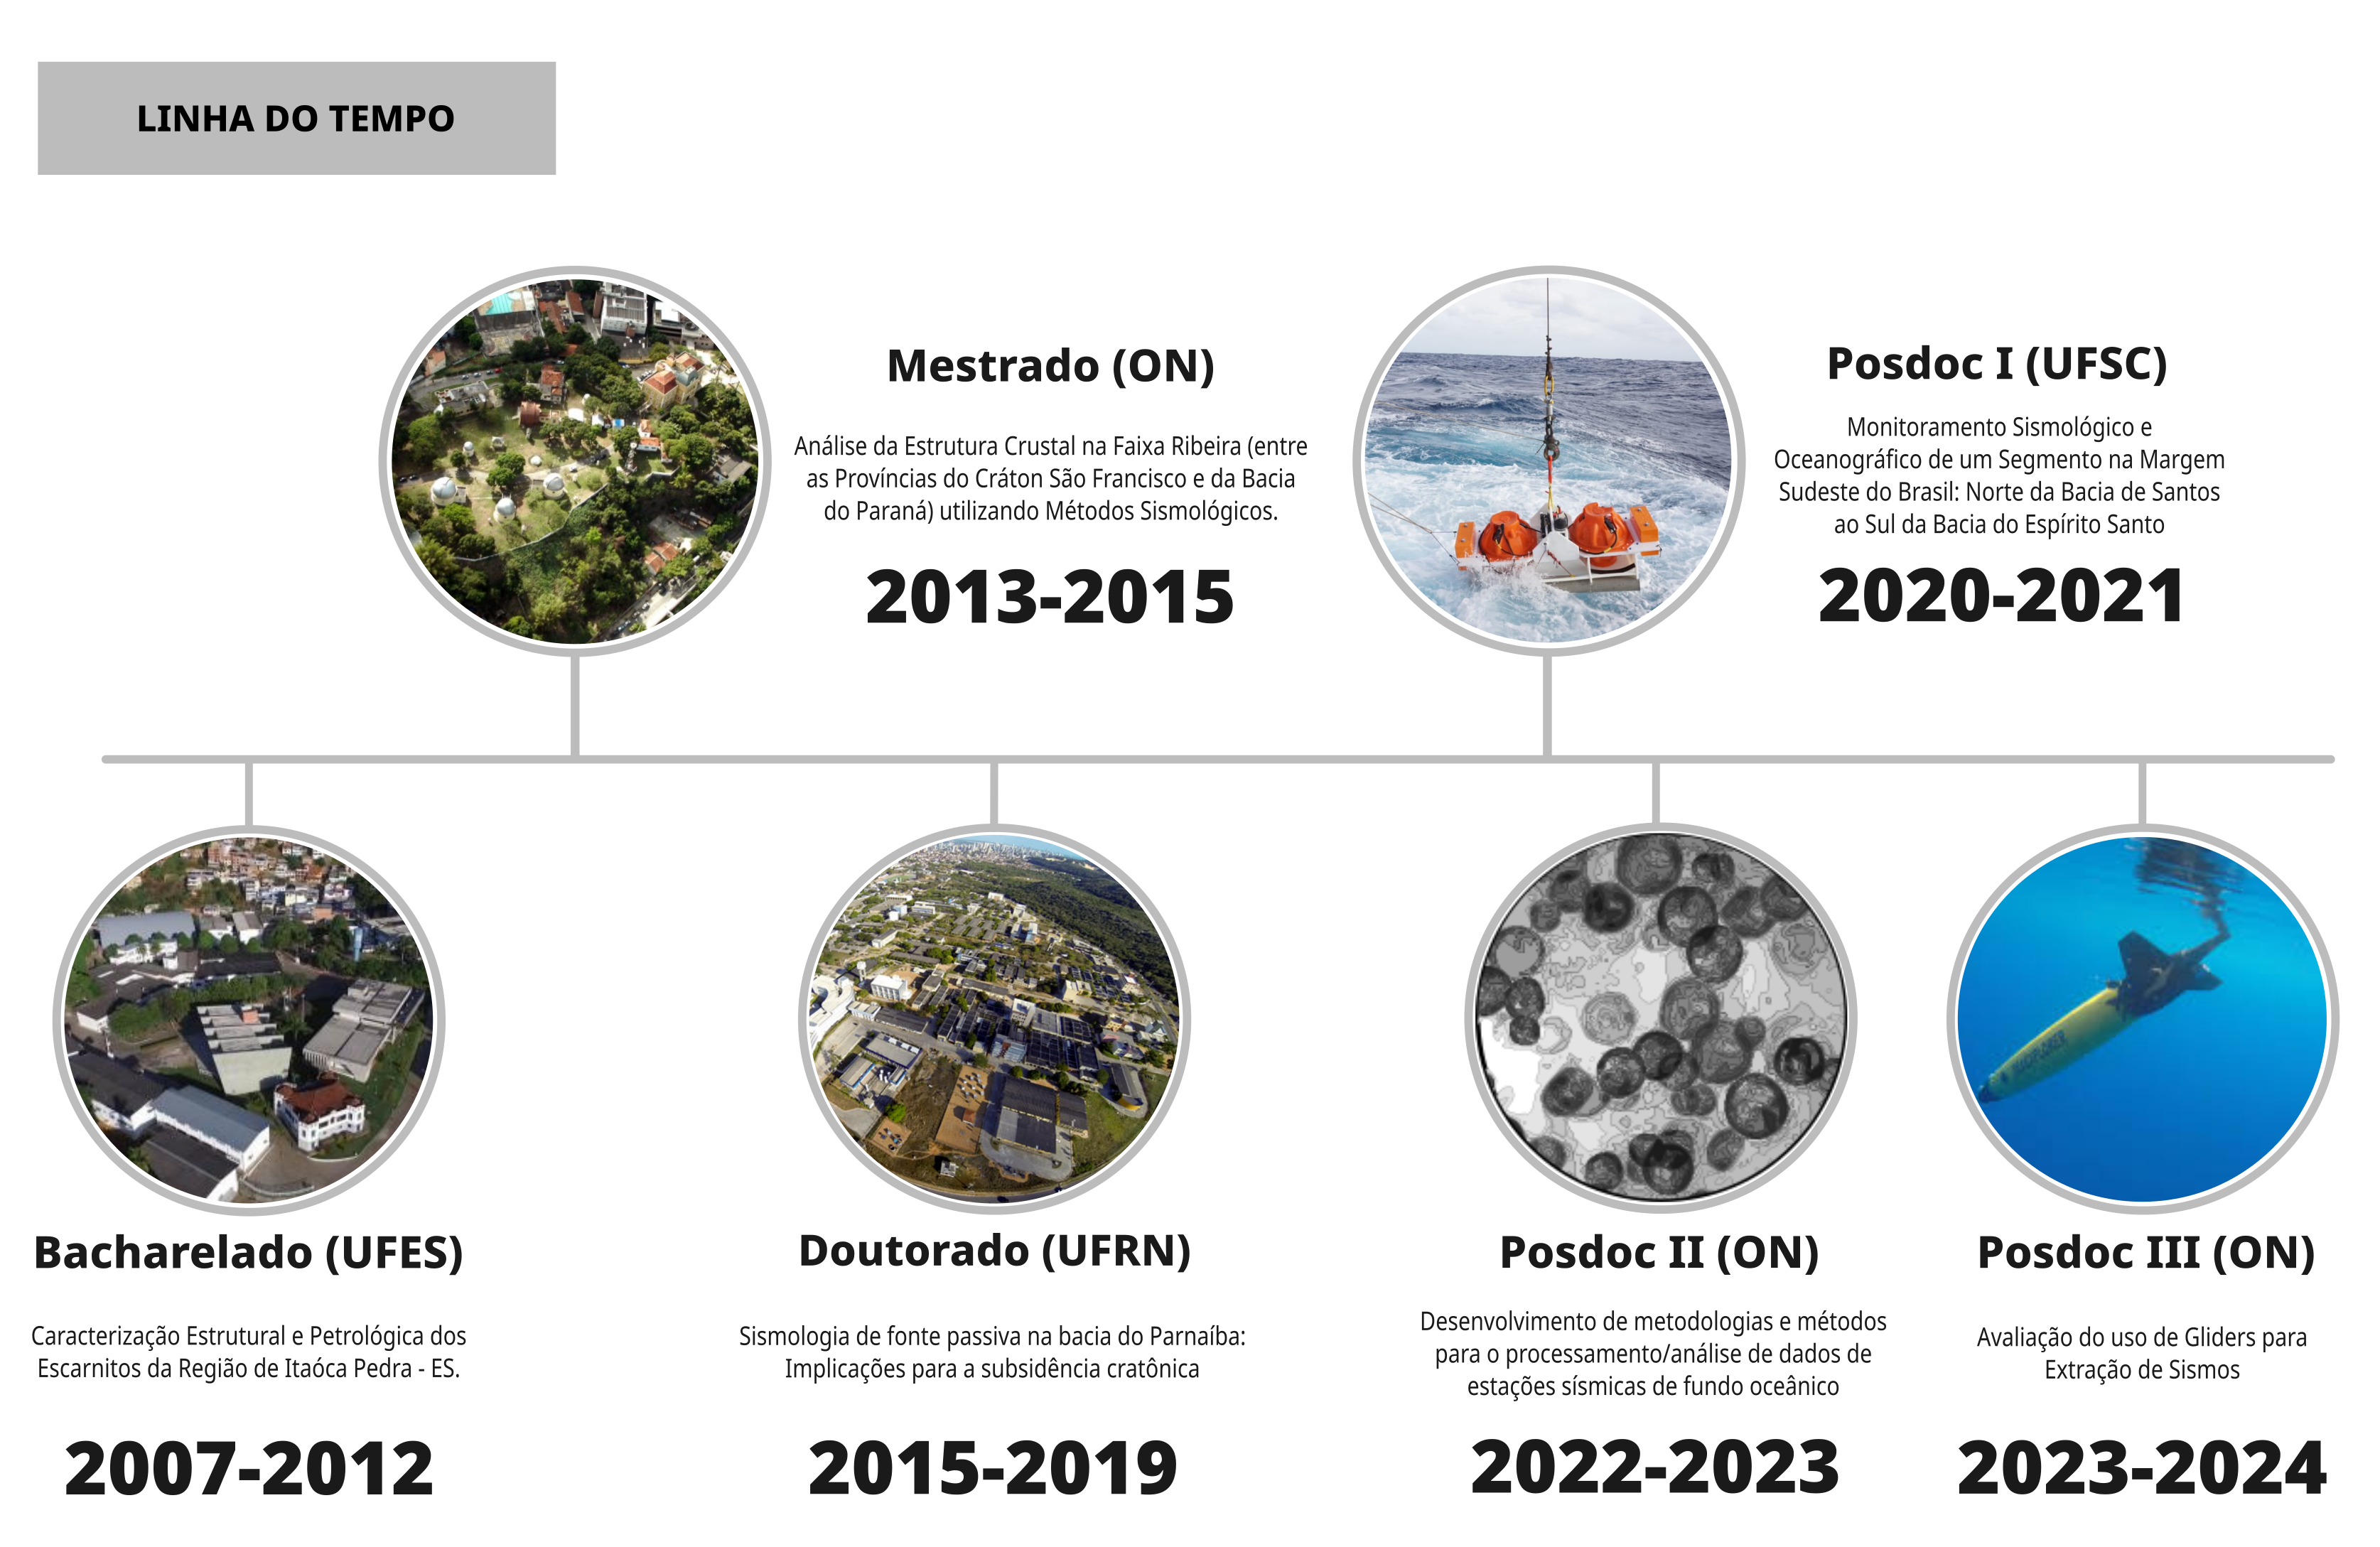
\includegraphics[width=\pagewidth]{images/linha_do_tempo.png}
  \end{center}
  \caption*{
    Resumo da minha trajetória acadêmica, desde a entrada na graduação em Geologia na Universidade Federal do Espírito Santo em 2007 até meu terceiro estágio pós-doutoral no Observatório Nacional no ano de 2024.
    }
\end{figure}
\end{landscape}
%==============================================================================
\tableofcontents

\mainmatter
\pagestyle{fancy}

%==============================================================================
\chapter{Apresentação}

\begin{figure}[h]
  \HeroFigPad
  \begin{center}
    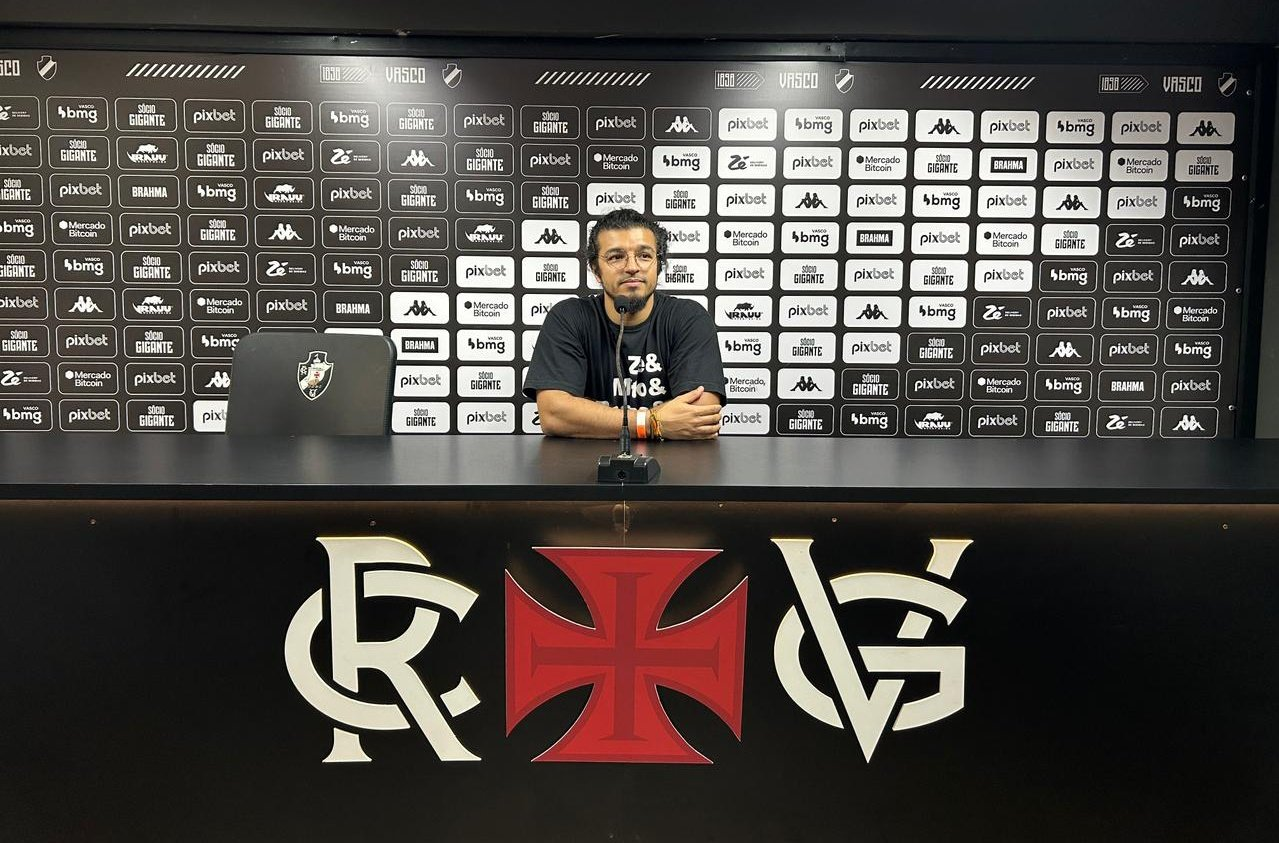
\includegraphics[width=\textwidth]{images/vasco.jpeg}
  \end{center}
  \caption{
    Visitando em 2023 o estádio de \href{https://vasco.com.br/sao-januario/}{São Januário}, a colina histórica. Por estar localizada a menos de 1 km do Observatório Nacional, a sede do Vasco da Gama foi um dos principais fatores que me motivaram a entrar no programa de pós-graduação do Observatório Nacional.
  }
  \label{fig_riacho}
\end{figure}
\begin{summarybox}[frametitle=\faIcon{address-card}{}\quad Informações para contato]
  \begin{fa-ul}
    \faIcon{at} & email profissional: \href{mailto:\Email}{\Email} \\
    \faIcon{at} & email pessoal: \href{mailto:\EmailPersonal}{\EmailPersonal} \\
    \aiOrcid & ORCID: \href{https://orcid.org/\ORCID}{\ORCID} \\
    \aiResearchGate & ResearchGate: \href{\ResearchGate}{\ResearchGate} \\
    \aiLattes & Currículo Lattes: \url{https://lattes.cnpq.br/\Lattes} \\
    \faIcon{github} & Github: \url{https://github.com/diogoloc}
  \end{fa-ul}
\end{summarybox}

Este memorial apresenta uma análise sumária sobre a minha trajetória acadêmica, contemplando formação, atuação, atividades de ensino e divulgação/popularização da ciência.

\section{Juventude no interior}

Passei a maior parte da minha infância e juventude no extremo norte fluminense, mais precisamente em \href{https://www.itaperuna.rj.gov.br/pmi/}{Itaperuna}, próximo da tríplice fronteira entre os estados do Rio de Janeiro, Espírito Santo e Minas Gerais. Lá, vivenciei uma experiência comunitária singular que moldou profundamente minha perspectiva de vida. Apesar de, por vezes, sentir que isso poderia limitar meu futuro, a tranquilidade e a fraternidade do ambiente me fizeram encarar de maneira positiva todos os conselhos que recebi ao longo da vida, tanto da sabedoria dos mais velhos quanto dos sonhos dos jovens, que foram e são fundamentais em todos os movimentos que eu fiz durante a minha carreira acadêmica.

Vindo de uma família composta por 7 tios por parte de pai e 7 tios por parte de mãe, além de incontáveis primos, aprendi desde cedo a viver e compartilhar espaços com uma grande diversidade de idades, ideias e vivências. Além disso, a vida no interior criou laços de amizades profundos, adicionando ainda mais pessoas de diferentes credos a essa rica sopa cultural. Inspirado por exemplos de familiares, amigos e conhecidos, decidi no último ano ensino médio a aventurar-me em um curso superior, no caso em Geologia, pois era a combinação ideal para aplicar meus interesses e habilidades em matemática, geografia, computação e natureza. Essa escolha foi influenciada por diversos fatores: a paixão pela geografia da minha mãe, as histórias de lugares que meu pai visitou trabalhando, a sólida base em matemática adquirida na \href{https://qedu.org.br/escola/33001286-ce-dez-de-maio}{Escola Estadual 10 de Maio}, as incontáveis horas passadas nas lojas de videogames e as aventuras na natureza na roça do meu avô e nos acampamentos com amigos.

As aventuras vividas na juventude, aliadas à ética transmitida por familiares e amigos, constituíram os pilares fundamentais da minha carreira acadêmica e foram essenciais para nortear princípios relacionados à educação, ciência e inovação. Essa rede de apoio desempenhou um papel crucial ao me impulsionar a estabelecer objetivos e não temer propor novas metas, mesmo diante de desafios persistentes da minha formação.

%==============================================================================
\chapter{Formação Acadêmica}
\label{cap_formacao}

\begin{figure}[h]
  \HeroFigPad
  \begin{center}
    \includegraphics[width=\textwidth]{images/formacao.png}
  \end{center}
  \caption{
    Moisaco mostrando as diferentes fases da minha formação acadêmica. Esquerda: Realizando medidas estruturais no campo do trabalho de conclusão de curso na Serra de Itaóca Pedra-ES. Centro: Apresentação do seminário dos estudantes no Observatório Nacional. Instalação da estação sismográfica temporária na Bacia do Parnaíba (Maranhão) com o corpo técnico do \href{https://labsis.ufrn.br/}{LabSis-UFRN}.
  }
 \label{fig_formacao}
\end{figure}

\begin{summarybox}[frametitle=\faAward{}\quad Resumo da formação acadêmica]
  \begin{datelist}
    2007--2012 & Bacharelado em Geologia -- Universidade Federal do Espírito Santo \\
    2013--2015 & Mestrado em Geofísica -- Observatório Nacional \\
    2015--2019 & Doutorado em Geodinâmica e Geofísica -- Universidade Federal do Rio Grande do Norte
  \end{datelist}
\end{summarybox}

Este capítulo relata a minha trajetória acadêmica, da Graduação ao Doutorado, explorando alguns detalhes que foram cruciais na minha carreira e nos ajustes feitos durante o percurso.

\section{Universidade Federal do Espírito Santo}
\label{sec_ufrn}

\begin{subsummarybox}[frametitle=\faGraduationCap\quad Bacharelado em Geologia]
  \begin{fa-ul}
    \faFortAwesome & Universidade Federal do Espírito Santo (Alegre-ES) \\
    \faClock & Agosto 2007 -- Setembro 2012 \\
    \faUserTie & Orientador: Roberto Sacks de Campos\\
    \faChalkboardTeacher & Trabalho de conclusão: Caracterização Estrutural e Petrológica dos Escarnitos da Região de Itaóca Pedra - ES.
  \end{fa-ul}
\end{subsummarybox}


Depois algumas tentativas frustadas no vestibular do primeiro semestre de 2007, ingressei no curso de \href{https://geologia.ufes.br/}{Geologia} da \href{https://www.ufes.br/}{Universidade Federal do Espírito Santo} no segundo semestre de 2007. A combinação foi perfeita, já que o curso era na cidade de \href{https://alegre.es.gov.br/}{Alegre}, município do sul capixaba com uma população estimada de 30.000 habitantes, portanto era próximo a minha cidade natal e em uma cidade pacata, segura e com um custo de vida baixo, ideal para um universitário.

\subsection{Conteúdo básico: Ciências Exatas e Ambientais}
\label{sec_geo_basico}

Eu tive uma boa aderência ao conteúdo programático do curso, tanto nas disciplinas específicas da Geologia, como nas disciplinas básicas (e.g., Cálculo, Física, Geometria analítica, Físico-química I), mesmo com grandes deficiências em tópicos básicos de física, resultado de problemas crônicos no ensino médio das escolas públicas brasileiras. Seguindo o conselho do saudoso professor de Cálculo I e II \href{http://lattes.cnpq.br/8391815843000996}{Carlos Alberto Manfre}, decidi adicionar as disciplinas optativas de Cálculo III (ENG05506) e de Física III (ENG06034) para aprimorar meus conhecimentos na área. A última, ministrada pelo professor \href{http://lattes.cnpq.br/6503578618806955}{Roberto Colistete Júnior}, me impulsinou a estudar por conta própria a ligação da física com a geologia. No semestre seguinte, todo o conhecimento foi reforçado pela excelente disciplina de Geofísica Básica (ENG06501) ministrada pelo professor \href{http://lattes.cnpq.br/0799322864183147}{Welitom Rodrigues Borges}, fundamental para a minha escolha de seguir o estudo da Geofísica na pós-graduação. Um demonstrativo da melhora da minha base nas ciências exatas foi o convite para ser monitor da disciplina Físico-Química I (ENG05264) sob o comando da professora \href{http://lattes.cnpq.br/9146731989810239}{Raquel Vieira de Carvalho}.

\subsection{Conteúdo específico: Ciências Geológicas}
\label{sec_geo_especifico}

Na segunda parte do curso, resolvi me dedicar aos tópicos relacionados a tecnologia após receber o convite da professora e amiga \href{http://lattes.cnpq.br/9513837515797451}{Fabricia Benda de Oliveira} para participar como colaborador voluntário do projeto "Identificação e mapeamento de áreas de risco geológico no município de Alegre-ES" e para ser monitor voluntário da parte organizacional da disciplina de Mapeamento Geológico II (ENG06599). Devido a isso, adicionei várias disciplinas optativas relacionadas a \href{https://www.gov.br/economia/pt-br/assuntos/patrimonio-da-uniao/arquivos-anteriores-privados/programa-de-modernizacao/linha-do-tempo/34-sig-apostila.pdf}{Sistema de Informação Geográfica}, como Cartografia Temática e Digigal (ENG06786), Análise e Modelagem Espacial  (ENG06867) e Sistemas Globais de Geoposicionamento (ENG06945). O curso me forneceu a oportunidade de conhecer as regiões Sul, Sudeste, Centro-Oeste e Nordeste do Brasil em diversas aulas de campo. A excepcional junção da base teórica sólida com essa experiência prática foi extremamente inspiradora para a minha formação como geocientista. Após trocar experiências vividas na UFES com alunos de outras instituições mais consagradas da Geologia, eu vi o esforço herculiano meus dos professores para nos proporcionarem uma base teórica sólida e aulas de campo nos diversos contextos geológicos no Brasil. Essa é uma tarefa desafiadora para um curso recente, especialmente vinculado a um campus localizado em uma região interiorana de um pequeno estado brasileiro. Até hoje, eu continuo utilizando os conceitos que aprendi durante nas disciplinas do ciclo profissionalizante, como a excelente disciplina de Geologia Estrutural (ENG06600) ministrada pelo professor \href{http://lattes.cnpq.br/1004206862799097}{Fernando Jacques Althoff} e Geologia do Brasil pelo professor \href{http://lattes.cnpq.br/5883057974133630}{Felipe Guadagnin}. Durante o trabalho de conclusão de curso (TCC) utilizei os conceitos de todas essas disciplinas como também das disciplinas proferida pelo meu orientador \href{http://lattes.cnpq.br/5081674111092263}{Roberto Sacks de Campos}, como Geoquímica (ENG06506) e Petrologia Metamórfica (ENG06865). A elaboração do TCC, entitulado \href{https://doi.org/10.6084/m9.figshare.25366483.v1}{Caracterização Estrutural e Petrológica dos Escarnitos da Região de Itaóca Pedra - ES}, foi muito uma experiência muito enriquecedora, pois organizei as viagens de campo, a preparação das lâminas e todo o calendário de execução das etapas de forma independente. Todo esse trabalho foi crucial para compreender que o processo de concepção e implementação de um projeto é um empreendimento extenso e requer dedicação intensa.

\subsection{Bolsa de Pesquisa (2011-2012)}
\label{sec_bolsa_hidro}

\begin{summarybox}[frametitle=\faProjectDiagram{}\quad Resumo do projeto]
  \begin{datelist}
    \faFile* & Levantamento Hidrogeológico do Estado do Espírito Santo \\
    \faHammer & Universidade Federal do Espírito Santo e Universidade Federal do Ceará \\
    \faCalendar*[regular] & 24 meses \\
    \faMapMarked* & 37 municípios dos Espírito Santo \\
    \faUserTie & Paulo de Tarso Ferro de Oliveira Fortes \\
    \faWallet & Petrobras \\
    \faMoneyBill*[regular] & R\$ 3.447.638,38
  \end{datelist}
\end{summarybox}

No segundo semestre de 2011, durante meu último ano de graduação, fui aprovado no processo seletivo para bolsista no projeto de Pesquisa \& Desenvolvimento \href{https://contratos.ufes.br/sites/contratoseconvenios.ufes.br/files/field/anexo/projeto_basico462015.pdf}{Levantamento Hidrogeológico do Estado do Espírito Santo}, desenvolvido em conjunto pela Universidade Federal do Espírito Santo e pela Universidade Federal do Ceará e coordenado pelo professor \href{http://lattes.cnpq.br/5417271870207313}{Paulo de Tarso Ferro de Oliveira Fortes}. Tal projeto tinha a finalidade de caracterizar regionalmente o potencial hídrico dos aqüíferos e reservatórios rasos das províncias sedimentares e cristalinas localizadas em 37 municípios no estado do Espírito Santo, visando a explotação racional destes recursos para sua utilização em usos diversificados. O projeto foi executado com recursos financeiros da Petrobras, onde eu recebia uma bolsa através da \href{https://mapaosc.ipea.gov.br/detalhar/1246897}{Fundação Ceciliano Abel de Almeida (FCAA)} para executar os seguintes objetivos:

\begin{itemize}
  \item Organização da base cartográfica digital das folhas topográficas Linhares, Rio Doce, Baixo Guandu, Colatina, Montanha e Nanuque (IBGE - 1:100.000);
  \item Desenvolvimento de atividades de campo no período de 13-18/02/2012 visando ao cadastramento de poços tubulares profundos.
\end{itemize}

A participação neste projeto foi um marco na minha trajetória acadêmica, pois era uma grande equipe de alunos trabalhando em conjunto. A experiência me proporcionou a chance única de explorar o interior da região norte do Espírito Santo, conhecendo de um outro ângulo as características culturais e geográficas locais. Ao testemunhar de perto a execução de um projeto de grande envergadura, fui capaz de absorver valiosos ensinamentos e aprender com a prática, aprimorando assim minha compreensão sobre a implementação eficaz de iniciativas desse porte.

\subsection{Bolsa de Estágio (2012)}
\label{sec_bolsa_petro}

\begin{summarybox}[frametitle=\faInfoCircle{}\quad Resumo do estágio]
  \begin{datelist}
    \faFile* & Estágio Supervisionado em Geologia \\
    \faCalendar*[regular] & 3 meses (Junho a Agosto) \\
    \faMapMarked* & E\&P-SERV/US-SUB/GM (Geologia Marinha/Macaé-RJ) \\
    \faUserTie & Marco Aurélio de Campos Merschmann \\
    \faWallet & Petrobras
  \end{datelist}
\end{summarybox}

No final do primeiro semestre de 2012, fui selecionado no processo seletivo para estagiário na Unidade de Serviços Submarinos da \href{https://petrobras.com.br/}{Petrobras}, mais precisamente na gerência de Geologia Marinha, que na época era chefiada pelo geofísico \href{https://br.linkedin.com/in/marco-aur\%C3\%A9lio-merschmann-b9381823}{Marco Aurélio de Campos Merschmann}. O estágio foi realizado na Petrobras S.A., localizada no município de Macaé, no estado do Rio de Janeiro. O plano de trabalho englobava atividades nas bases de Imboassica, setor de Geologia Marinha, e Imbetiba, laboratório de Sedimentologia e Estratigrafia. Os objetivos propostos para o estágio foram:

\begin{itemize}
  \item Acompanhamento de mapeamento de dados sísmicos 3D e  de alta freqüência;
  \item Acompanhamento da descrição de testemunhos geológicos (Laboratório de Sedimentologia);
  \item Acompanhamento da elaboração de Laudos para subsidiar a perfuração de poços, instalação de equipamentos submarinos e dutos;
  \item Leitura e análise de conteúdo dos relatórios de Estudos de
Geohazard.
\end{itemize}

A primeira dificuldade encontrada foi na sistemática corporativa empregada pela Petrobras, principalmente no grande número de siglas e equipamentos utilizados. No entanto, a partir do estudo dos laudos técnicos e de esclarecimentos pontuais por parte da equipe de técnicos, a adaptação evoluiu em um ritmo acelerado. Este estágio foi muito proveitoso para entender o funcionamento de uma grande empresa do setor energético, principalmente conhecer as rotinas de trabalho utilizadas pelos técnicos da Geologia Marinha para armazenar, carregar, modelar, calcular e converter dados geológicos e geofísicos. Outro trabalho que foi um diferencial nesse estágio foi a abertura, descrição, documentação, datação e interpretação de testemunhos geológicos. Vale destacar que graças a disciplina optativa Geologia do Quaternário (ENG05572), ministrada pelo professor \href{http://lattes.cnpq.br/6157185791642499}{Cláudio Eduardo Lana}, pude acompanhar sem problemas o trabalho no Laboratório de Sedimentologia, o que não era comum, pois é uma área muito específica nas ciências geológicas.

Avaliando todos os pontos presenciados durante este período, tanto positivos quanto negativos, posso atestar que essa experiência foi bastante proveitosa na minha carreira, englobando experiências no campo relacional (gestão de pessoas) e no campo intelectual (contato direto com o estado da arte na tecnologia do setor de petrolífero).

\section{Observatório Nacional}
\label{sec_on}

\begin{subsummarybox}[frametitle=\faGraduationCap{}\quad Mestrado em Geofísica]
  \begin{fa-ul}
    \faFortAwesome & Observatório Nacional (Rio de Janeiro-RJ) \\
    \faClock & Março 2012 -- Abril 2015 \\
    \faUserTie & Stéphane Gérard Martial Drouet\\
    \faUserTie & Bruno Yann Nicolas Goutorbe\\
    \faWallet & Conselho Nacional de Desenvolvimento Científico e Tecnológico - CNPQ \\
    \faChalkboardTeacher & Dissertação: Análise da Estrutura Crustal na Faixa Ribeira (entre as Províncias do Cráton São Francisco e da Bacia do Paraná) utilizando Métodos Sismológicos.
  \end{fa-ul}
\end{subsummarybox}

Ainda no estágio, conversando com os geólogos e geofísicos da gerência de Geologia Marinha, fui alertado sobre as vantagens de continuar os estudos e entrar em uma instituição de pesquisa científica. Observando o benefício da exposição a uma diversidade de formas de pensamento oriunda de diferentes locais e instituições, decidi que estava na hora de mudar minha realidade, indo para uma metrópole e uma instituição de pesquisa consagrada no Brasil. Devido a fatores logísticos e operacionais, o \href{https://www.gov.br/observatorio/pt-br}{Observatório Nacional (ON)} despertou meu interesse. No final de 2012 prestei concurso para o \href{https://www.gov.br/observatorio/pt-br/assuntos/programas-academicos/pos-graduacao-em-geofisica}{Programa de Pós-graduação em Geofísica do ON} e no começo de março de 2013 iniciei os estudos. Mesmo não tendo um orientador e um projeto no início do mestrado, eu estava convencido que trabalharia com algum tema relacionado a Terra Sólida. Após algumas tratativas, iniciei o projeto de mestrado com o professor \href{http://lattes.cnpq.br/0563544084744404}{Stéphane Gérard Martial Drouet} com dados estações sismográficas temporárias de banda larga instaladas no Sudeste do Brasil.

O ambiente da pós-graduação do ON era extremamente diverso e cientificamente estimulante, pois as salas mesclavam doutorandos e mestrandos de diversas áreas da geofísica e astronomia. A multiculturalidade era gigantesca. Devido a isso, o ambiente era acolhedor e as conversas informais eram cheias de conselhos. Essas dicas informais foram fundamentais para o meu crescimento como cientista. Como eu sou oriundo da Geologia, eu tinha muita experiência prática nas geociências, no entanto, eu tinha uma conhecimento teórico muito raso. Graças as conversas com os físicos, geólogos e geofísicos, tantos que seria indelicado tentar citar neste texto, eu iniciei os estudos de inversão e programação em \href{https://www.python.org/}{python}, além das dicas essencias para um processamento correto dos dados nas disciplinas de problemas inversos, ministradas pelos professores \href{http://lattes.cnpq.br/4332841435949533}{Vanderlei Coelho de Oliveira Junior} e \href{http://lattes.cnpq.br/0391036221142471}{Valéria Cristina Ferreira Barbosa}. Somado a isso, fui incentivado a retrabalhar os dados oriundos do meu trabalho de conclusão de curso utilizando métodos aeromagnetométricos e aeroradiométricos para correlacionar com o mapeamento geológico realizado. Com isso, no primeiro semestre do mestrado eu publiquei um resumo expandido, entitulado \href{https://doi.org/10.1190/sbgf2013-129}{Aerogeophysical data to refine geological mapping: A semi-quantitative approach}, no 13th Congresso Internacional da Sociedade Brasileira de Geofísica entre 26 e 29 de Agosto 2013. Mesmo não pertecendo a nenhum projeto, o programa de pós-gradução em Geofísica do ON me forneceu diversas oportunidades de frequentar congressos nacionais e internacionais, onde pude aprimorar minhas vacâncias na pesquisa científica.

Meu projeto de mestrado, sob a orientação do professor Stéphane Drouet, era a análise e delimitação de grandes feições estruturais crustais através dos resultados de duas metodologias distintas: Função do Receptor de onda P e Tomografia de Ruído Sísmico Ambiental (momento que o professor \href{http://lattes.cnpq.br/5754348793953158}{Bruno Yann Nicolas Goutorbe} entrou como co-orientador no mestrado). Os dados era oriundos de estações temporárias do projeto \href{http://www.pegbr.on.br:8080/pegbr/visualizar/SolicitacaoDadosProjeto.jsp?cod=74}{SUBSAL} e estações permanentes da \href{www.rsbr.on.br}{Rede Sismográfica Brasileira}. Os resultados oriundos das Funções do Receptor foram apresentadados em um resumo expandido, entitulado \href{http://dx.doi.org/10.22564/6simbgf2014.043}{Analysis of Crustal Structure in the region of Ribeira Belt (between the Provinces of the São Francisco Craton and the Paraná Basin) using Seismological Methods}, enviado para o VI Simpósio Brasileiro de Geofísica entre 14 e 16 de Outubro de 2014. Devido à excelente sintonia entre meus orientadores e eu, o professor Bruno Goutorbe me convidou para colaborar na interpretação dos resultados provenientes da Tomografia de Ruído obtidos a partir de 53 estações sismográficas permanentes espalhadas pelo território brasileiro no período de 1996 a 2012. O trabalho entitulado \href{http://dx.doi.org/10.1093/gji/ggv343}{Rayleigh wave group velocities at periods of 6–23 s across Brazil from ambient noise tomography} foi publicado no segundo semestre de 2015. Terminei meu mestrado em abril de 2015 e iniciei o processo de entrada no Doutorado em Geofísica do Observatório Nacional, no entanto, por ironia do destino, os meus orientadores não permaneceram no Brasil e eu tive que reajustar a direção da minha carreira.

\section{Universidade Federal do Rio Grande do Norte}
\label{sec_doutorado}

\begin{subsummarybox}[frametitle=\faGraduationCap{}\quad Doutorado em Geodinâmica e Geofísica]
  \begin{fa-ul}
    \faFortAwesome & Universidade Federal do Rio Grande do Norte  (Natal-RN)  \\
    \faClock & Agosto 2015 -- Dezembro 2019 \\
    \faUserTie & Jordi Julià Casas \\
    \faWallet & Fundação Norte-Rio-Grandense de Pesquisa e Cultura - FUNPEC \\
    \faChalkboardTeacher & Tese: Sismologia de fonte passiva na bacia do Parnaíba: Implicações para a subsidência cratônica.
  \end{fa-ul}
\end{subsummarybox}

\begin{summarybox}[frametitle=\faProjectDiagram{}\quad Resumo do projeto]
  \begin{datelist}
    \faFile* & Parnaíba Basin Analysis Project (PBAP) \\
    \faHammer & Universidade Federal do Espírito Santo e Universidade Federal do Ceará \\
    \faCalendar*[regular] & 2012 - 2017 \\
    \faMapMarked* & Bacia do Parnaíba \\
    \faUserTie & Jordi Julià Casas \\
    \faWallet & BP Energy do Brasil LTDA  \\
    \faMoneyBill*[regular] & R\$ 1.998.038,98
  \end{datelist}
\end{summarybox}

Após a finalizar o mestrado e ser notificado que não teria mais a possibilidade de continuar como aluno da área de Sismologia no ON, optei por mudar de instituição para me manter na área e aprimorar os estudos sismológios. No mestrado eu tive uma formação sólida como geofísico, no entanto, carecia de estudos profundos em tópicos específicos da Sismologia. Conversando com professores, recebi uma notificação que abrira uma vaga para doutorado no \href{https://posgraduacao.ufrn.br/325}{Programa de Pós-Graduação em Geodinâmica e Geofísica} da UFRN na área de Sismologia com o professor \href{http://lattes.cnpq.br/0012168139768170}{Jordi Julià Casas}. Conversando novamente com familiares e amigos, decidi que seria interessante viver uma nova experiência no Nordeste do Brasil. Com isso, em agosto de 2015, me mudei para Natal-RN, para novamente mudar minha realidade, indo para uma cidade localizada no extremo nordeste do país. Realmente, foi uma decisão acertada, pois a cidade é uma capital com cara de interior, onde o sol brilha o ano todo. 

Meu projeto de Doutorado foi financiado pelo PBAP, sendo um braço na busca da caracterização estrutural profunda da Bacia do Parnaíba através da sísmica passiva. As metodologias utilizadas, inversão conjunta e migração pré-empilhamento, tiveram a finalidade de expor as principais descontinuidades sísmicas na crosta e no manto para elucidar como o arcabouço geológico se comportou em meio aos processos geológicos que atuaram abaixo da bacia do Parnaíba. No primeiro ano do doutorado eu me dediquei aos estudos das diversas disciplinas envolvendo tópicos da Sismologia. Além disso, como mostrado na Figura \ref{fig_formacao}, no primeiro ano do Doutorado eu me dediquei à implantação do perfil de estações sismográficas temporárias na Bacia do Parnaíba, sendo que a última estação instalada estava localizada a aproximadamente 2000 km de distância de Natal-RN. Todo este percurso foi realizado em seguidas viagens de carro, onde pude vivenciar todo o trabalho realizado pelos técnicos do LabSis-UFRN para manter em funcionamento a \href{https://labsis.ufrn.br/}{Rede Sismográfica do Nordeste (RSISNE)}. As longas viagens foram proveitosas para também criar um vínculo com os técnicos do laboratório, principalmente com \href{http://lattes.cnpq.br/0406798380417692}{Eduardo Alexandre Santos de Menezes}, quando em uma conversa sobre uma boa metodologia para atestar de qualidade de uma estação sísmográfica, confeccionamos o trabalho \href{https://dx.doi.org/10.6084/m9.figshare.25367143}{Assessing data quality and station performance for eight meridian compact posthole stations deployed in the parnaíba basin}, que foi apresentado no II Simpósio Brasileiro de Sismologia entre 12 a 15 de novembro de 2017. Este trabalho gerou um conjunto de códigos\footnote{Python framework for analysing the quality of seismological data archived in based on ObsPy em \url{https://github.com/dIOGOLOC/codes_escritos/tree/b0f5c54cf46a37c2642732c47bcb422bf00495fd/LabSis_controle_de_qualidade}} que o LabSis utiliza para o controle de qualidade dos seus equipamentos.  

Os resultados da tese apresentaram metodologias diferentes para caracterizar a estrutura crustal e da parte mais rasa do manto superior abaixo da Bacia do Parnaíba e para imagear a Zona de Transição do Manto (limite entre o manto superior e o manto inferior). Na primeira parte, os métodos utilizados estimaram pontualmente a espessura da crosta e a razão Vp/Vs nas estações sismográficas de banda larga sobre a bacia. Juntamente com essas estimativas foram recuperados perfis de velocidade da onda S em função da profundidade através de uma inversão conjunta de dados sismológicos. Os resultados desses estudos foram bem relevantes e foram apresentados em conferências nacionais\footnote{Anais do 48º Congresso Brasileiro de Geologia, 2016, Porto Alegre em \url{http://cbg2017anais.siteoficial.ws/ste01/ID5293_110479_52_48CBG_Diogo.pdf}} e internacionais\footnote{19th EGU General Assembly, EGU2017, proceedings from the conference held 23-28 April, 2017 in Vienna, Austria., p.10252 em \url{https://ui.adsabs.harvard.edu/abs/2017EGUGA..1910252C/abstract}}. Estes resultados estavam em sintonia com outros métodos geofísicos realizados sobre o mesmo perfil, então no primeiro semestre de 2018, o primeiro artigo do doutorado foi publicado com o título \href{https://doi.org/10.1144/SP472.8}{Deep crustal architecture of the Parnaíba basin of NE Brazil from receiver function analysis: implications for basin subsidence}.

Dois eventos foram muito marcantes no meu doutorado, o primeiro, em meados de 2016 participei da \href{https://indico.ictp.it/event/7615/material/11/0.jpg}{School on Seismology beyond Textbooks} entre 29 de Agosto e 3 Setembro de 2016 no Centro Internacional de Física Teórica em Trieste-IT. Nesta escola eu pude ter um encontro com diversos doutorandos ao redor do mundo, além de interagir com grandes cientistas na área da Sismologia Moderna, como é o exemplo do professor \href{https://scholar.google.fr/citations?user=ZCRP01AAAAAJ&hl=fr}{Michel Campillo}, do qual eu utilizei a metodologia para fazer os trabalhos sobre Tomografia de Ruído Sísmico. O segundo evento marcante foi em meados de 2017 o \href{https://geodynamics.org/events/details/218}{CIG-LLNL Computational Seismology Workshop} no Laboratório Nacional Lawrence Livermore na Califórnia, um fato interessante é que o laboratório é um dos dois únicos lugares onde são projetadas as ogivas nucleares nos Estados Unidos da América. O objetivo do workshop foi fornecer aos participantes uma experiência prática no acesso, processamento, modelagem e visualização de dados sísmicos usando ferramentas avançadas em Sismologia em um supercomputador. A partir dessas experiências retornei a Natal-RN com um novo pensamento, o qual precisa aprimorar as minhas rotinas de programação criadas para processar os dados. 

A partir do segundo ano de doutorado, iniciei o processo que mudou a minha formação, todo programa que eu fosse utilizar, eu teria que criar um pacote de códigos estruturados e de fácil reprodutibilidade. Com isso, iniciei os estudos sobre a Zona de Transição do Manto e sobre o processo de migração das Funções do Receptor. Após um longo período estudando e programando, eu criei um pacote\footnote{Python framework for receiver functions migration em \url{https://github.com/dIOGOLOC/codes_escritos/tree/b0f5c54cf46a37c2642732c47bcb422bf00495fd/mantle_transition_zone_migration_obspy_Pds}} que migra as formas de onda de tempo para profundidade e com os resultados foi possível avaliar o papel de processos convectivos profundos e heterogeneidades do manto na formação e evolução da Bacia do Parnaíba. Novamente foi um salto muito grande na minha caminhada acadêmica investigar as descontinuidades mantélicas, pois é natural para um geólogo entender a estrutura da Crosta da Terra porque é visível, porém o arcabouço do Manto estava totalmente fora da minha zona de conforto. Nossos resultados mostraram que a espessura da zona de transição se mantém constante sob a bacia, isto é, não existe nenhuma evidência nesta camada de um fluxo vertical negativo pretérito ou heterogeneidade mantélica que possa ter influenciado no processo de formação da bacia. O artigo entitulado "Mantle transition zone topography beneath the Parnaíba basin of NE Brazil: New constraints on deep mantle dynamics" foi submetido em 2019 à revista Geophysical Journal International e obteve um parecer positivo para publicação após correções relativamente pequenas. No entanto, devido a problemas de cunho pessoal e situações da pandemia que se iniciou no começo de 2020, eu não continuei com a submissão. Creio que foi uma decisão acertada, pois estou reformulando novamente o artigo. Atualizando o banco de dados para 2024, agora tenho resultados e discussões mais sólidas.

%==============================================================================
\chapter{Atuação Profissional}
\label{cap_atuacao}

\begin{figure}[h]
  \HeroFigPad
  \begin{center}
    \includegraphics[width=\textwidth]{images/atuacao_pos.png}
  \end{center}
  \caption{
    Moisaico mostrando as diversas frentes de atuação durante o período do estágio pós-doutoral no Observatório Nacional. Primeira: Recebendo e apresentando os equipamentos utilizados nas campanhas de aquisição de dados no fundo oceânico à Diretoria de Desenvolvimento Científico e Tecnológico da \href{http://www.finep.gov.br/}{FINEP} (Financiadora de Estudos e Projetos). Segunda: Recebendo o engenheiro da Güralp para a manuntenção dos Sismômetros de Fundo Oceânico. Terceira: Representante da comitiva da RSBR na empresa francesa \href{https://www.linkedin.com/company/osean-sas}{OSEAN} para aquisição dos Sismógrafos flutuantes (\href{https://www.geoazur.fr/GLOBALSEIS/Mermaid.html}{MERMAID}). Quarta: Apresentação de trabalho científico no 18th International Congress of the Brazilian Geophyisical Society and EXPOGEf.}
\end{figure}

\begin{summarybox}[frametitle=\faInfoCircle{}\quad Resumo da atuação profissional]
  \begin{datelist}
    2020--2021 & Estágio Pós-doutoral -- Universidade Federal de Santa Catarina \\
    2022--2023 & Estágio Pós-doutoral -- Observatório Nacional \\
    2023--atual & Estágio Pós-doutoral -- Observatório Nacional \\
  \end{datelist}
\end{summarybox}

Este capítulo relata minha atuação profissional, tanto no estágio pós-doutoral nas instituições de ensino e pesquisa, quanto como voluntário em atividades de divulgação e popularização da ciência, buscando diminuir o espaço entre a sociedade e as instituições de pesquisa. Os relatos abaixo se referem à atividades institucionais, experiências pessoais, formação de capital humano e atividades de ensino.

\section{Universidade Federal de Santa Catarina (2020-2021)}
\label{sec_ufsc}

\begin{subsummarybox}[frametitle=\faUniversity{}\quad Vínculo institucional]
  \begin{fa-ul}
    \faUser & Estágio pós-doutoral \\
    \faMapMarker & Department of Earth Sciences -- School of Ocean and Earth Science and Technology\\
    \faCalendar & Fevereiro 2017 -- Agosto 2019
  \end{fa-ul}
\end{subsummarybox}


\section{Observatório Nacional (2022-2023)}
\label{sec_ufsc}

\begin{subsummarybox}[frametitle=\faUniversity{}\quad Vínculo institucional]
  \begin{fa-ul}
    \faUser & Estágio pós-doutoral \\
    \faMapMarker & Department of Earth Sciences -- School of Ocean and Earth Science and Technology\\
    \faCalendar & Fevereiro 2017 -- Agosto 2019
  \end{fa-ul}
\end{subsummarybox}


\section{Observatório Nacional (2023-atual)}
\label{sec_ufsc}

\begin{subsummarybox}[frametitle=\faUniversity{}\quad Vínculo institucional]
  \begin{fa-ul}
    \faUser & Estágio pós-doutoral \\
    \faMapMarker & Department of Earth Sciences -- School of Ocean and Earth Science and Technology\\
    \faCalendar & Fevereiro 2017 -- Agosto 2019
  \end{fa-ul}
\end{subsummarybox}

\chapter{Popularização da Ciência}
\label{chap_comunidade}

\bigskip

\begin{figure}[h]
  \HeroFigPad
  \begin{center}
    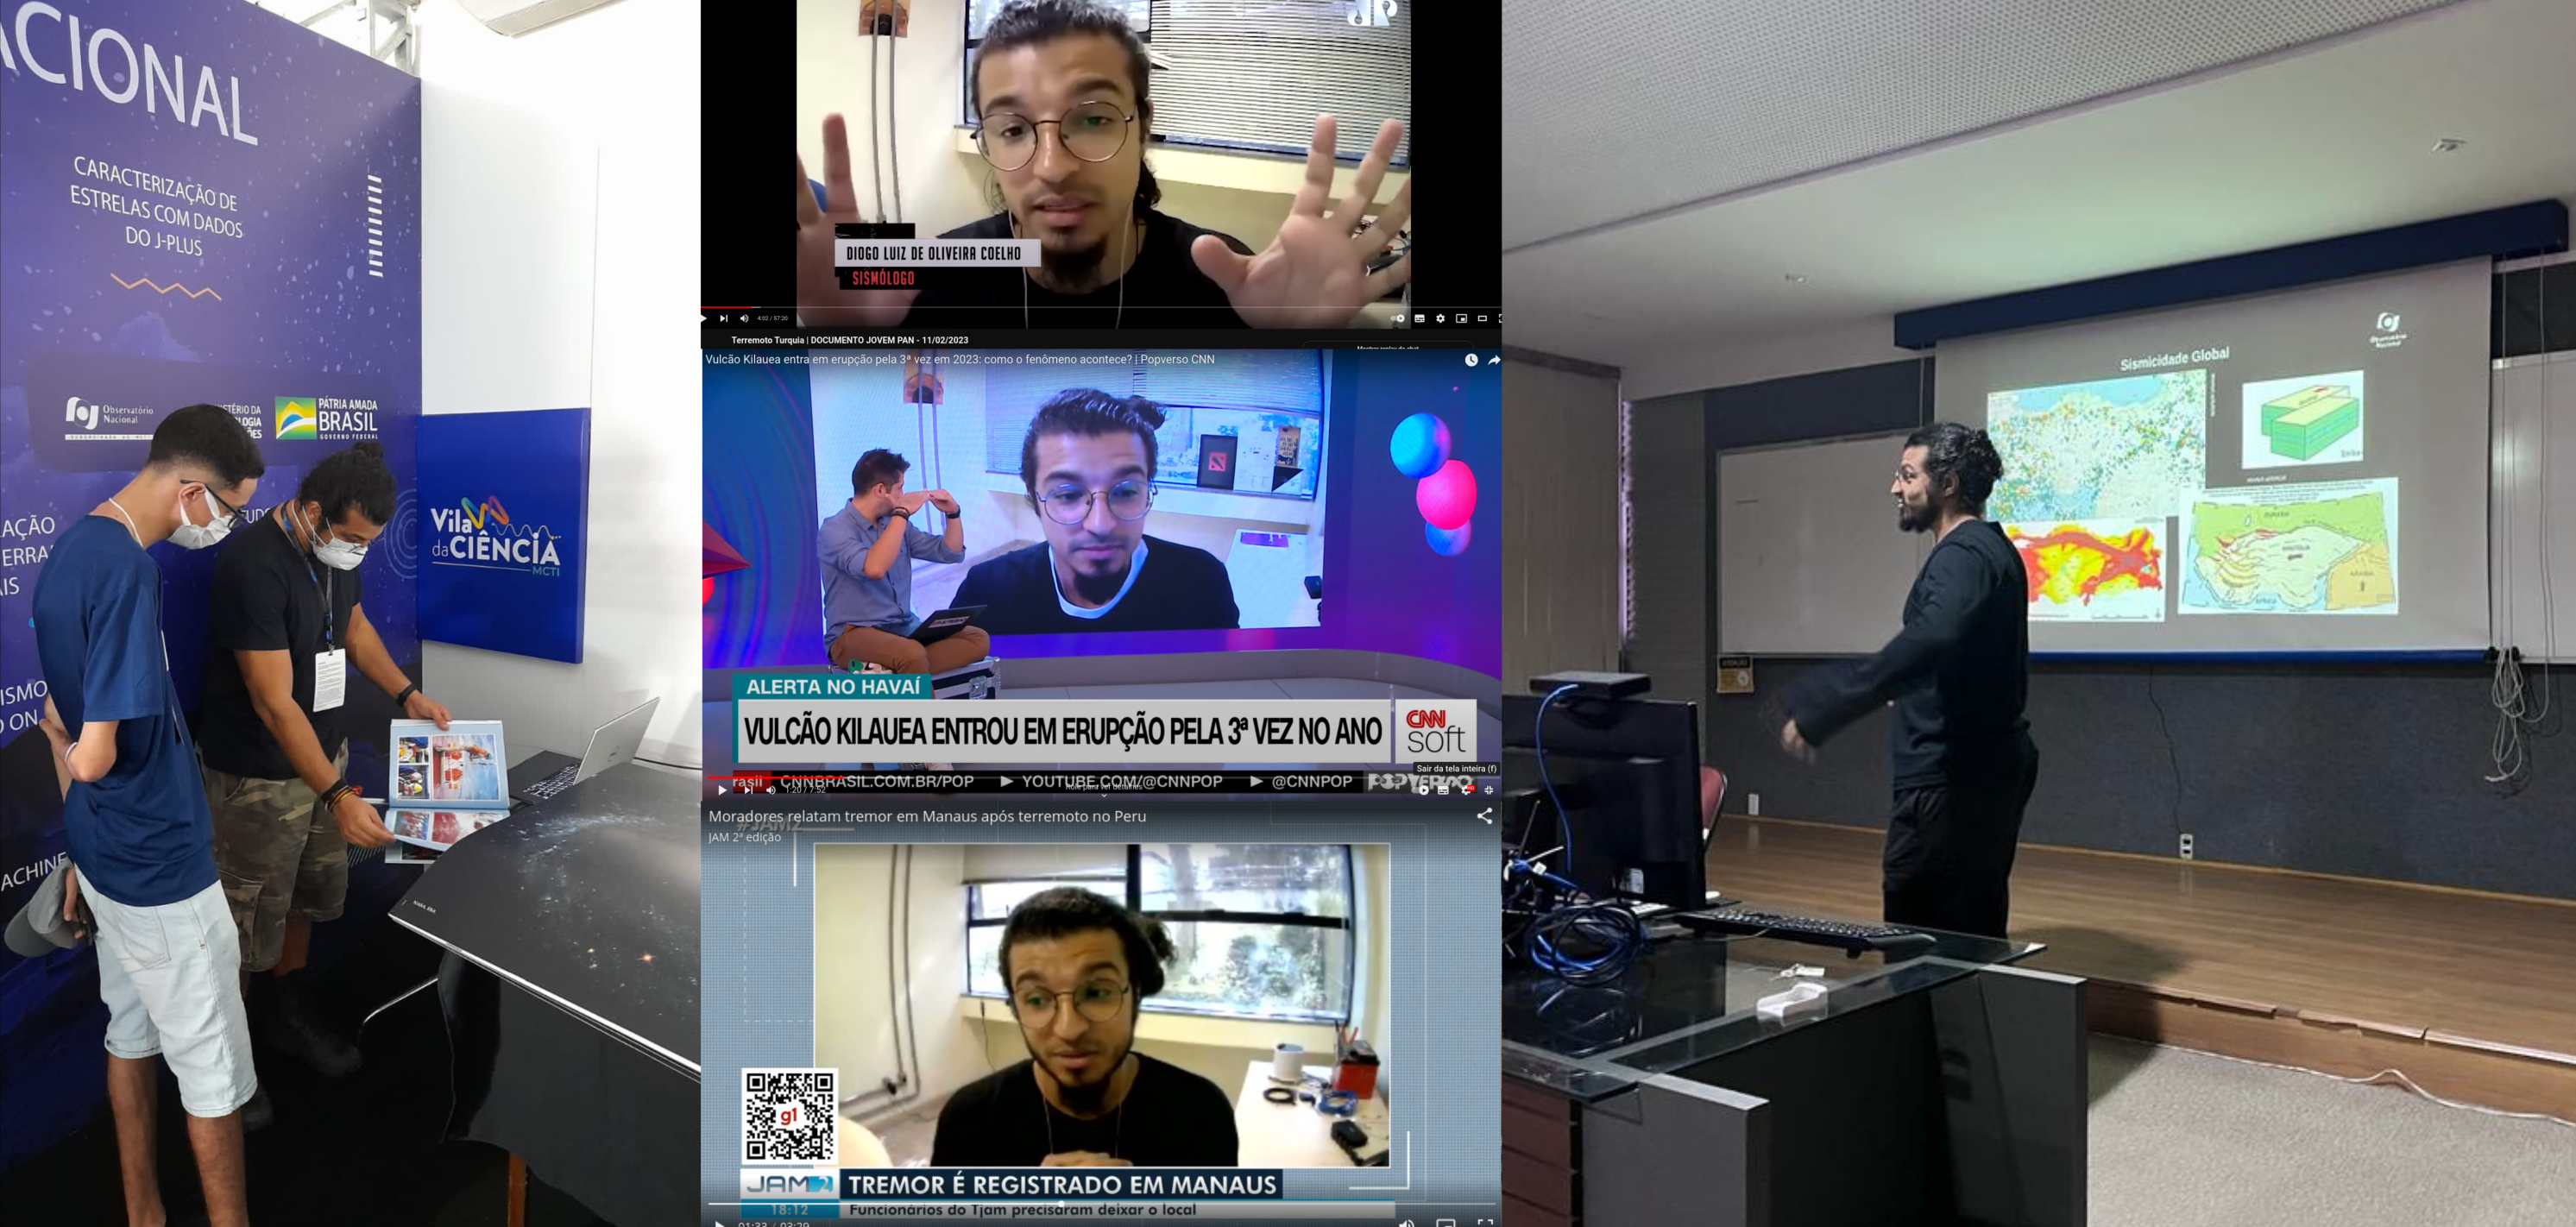
\includegraphics[width=\textwidth]{images/atuacao_divulga.png}
  \end{center}
  \caption{
    Moisaico mostrando as diversas frentes de atuação na divulgação e popularização da ciência durante o estágio pós-doutoral no Observatório Nacional. Esquerda: Participação com o Projeto Sismo-oceanográfico em 2022 no Rio Innovation Week. Centro: 3 fotos de entrevistas respondendo os questionamentos da sociedade em relação a sismicidade brasileira e global. Direita: Ministrando o mini-curso “Sismologia: existem terremotos no Brasil?” na Universidade Federal de Pernambuco.}
\end{figure}

Após ingressar no estágio pós-doutoral, cerca de um mês depois, o planeta iniciou um extenso período de \href{http://repositoriocovid19.unb.br/repositorio-produtos/desvelando-o-isolamento-social-no-cotidiano-vivido-na-pandemia-da-covid-19/}{isolamento social}. Foi nesse contexto que constatei uma crescente demanda social por informações científicas, além de identificar uma lacuna significativa em minha carreira nesse campo tão crucial na ciência contemporânea. Diante dessa necessidade evidente, iniciei minhas atividades voltadas para à divulgação e popularização da ciência junto à Divisão de Comunicação e Popularização da Ciência (\href{https://www.gov.br/observatorio/pt-br/assuntos/areas-de-atuacao/divulgacao-e-popularizacao-da-ciencia}{DICOP}), reconhecendo a importância de fornecer conhecimento acessível à sociedade. Este capítulo relata minhas atividades relacionadas a divulgação da ciência, como mostra a Figura \ref{fig_resumo_divulgacao}. Durante esse período, meu engajamento abrangeu a diversas demandas da DICOP em variadas plataformas de comunicação, abordando tanto o meio virtual, por meio de redes sociais e canais de imprensa online, quanto atividades presenciais, como feiras e eventos de divulgação científica e tecnológica, assim que as restrições permitiram.

\begin{figure}
	\centering
	\begin{tikzpicture}
	\pie{34.3/Entrevista escrita (13),
		21.0/Entrevista gravada (8),
		10.5/Revisão de texto (4),
		7.8/Evento Online (3), 
		7.8/Entrevista ao vivo (3),
		5.2/Evento presencial (2),
		5.2/Mini-curso (2),
		8/Outros (3)}
	\end{tikzpicture}
	\caption{Estatística das atividades de divulgação científicas realizadas entre 2020 e 2024.}
	\label{fig_resumo_divulgacao}
\end{figure}

Os números apresentados acima, assim como a lista completa abaixo, fornecem uma visão detalhada dessa abordagem multifacetada na popularização da ciência e das atividades do Obseravtório Nacional ao longo do período que estive na instituição, um total de 38 atividades ao longo de 3 anos. Destaco que concedi dezenas de entrevistas, totalizando 24 (13 escritas, 8 gravadas e 3 ao vivo), contribuí revisando textos na temática da Sismologia e Geologia que foram publicados nas redes sociais do Obseravtório Nacional. Além disso, fiz parte da comitiva que participou do \href{https://www.gov.br/observatorio/pt-br/assuntos/areas-de-atuacao/divulgacao-e-popularizacao-da-ciencia/on-riw}{Rio Innovation Week}, o maior evento de tecnologia e inovação da América Latina, para apresentar as iniciativas, ações e projetos ligados ao \href{https://www.gov.br/mcti/pt-br}{MCTI}. Somada a isso, ministrei dois minicursos em duas instituições de ensino superior, na Universidade Federal do Espírito Santo para o curso de Geologia na \href{https://www.instagram.com/segeo.ufes/}{Semana de Estudos Geológicos da Universidade Federal do Espírito Santo} e no Instituto de Física da Universidade Federal de Pernambuco na \href{https://www.gov.br/observatorio/pt-br/assuntos/noticias/i-escola-itinerante-da-geofisica-do-observatorio-nacional-e-realizada-na-ufpe}{I Escola Itinerante da Geofísica do Observatório Nacional}. Ministrar um curso em outras instituições, não apenas promove a disseminação do conhecimento especializado, mas também desempenha um papel crucial na visibilidade e reputação do Observatório Nacional. Esses eventos compartilham expertise em contextos acadêmicos diversos, estabelecendo laços colaborativos e fortalecendo a presença no cenário acadêmico. Além disso, o envolvimento em eventos externos fortalece parcerias e colabora para o crescimento do programa de iniciação científica e pós-graduação do ON, estimulando a atração de novos alunos.

\bigskip

\begin{subsummarybox}[frametitle=\faList{}\quad Listagem das atividades de divulgação científica]
  \begin{datelist}
  	06/05/2020 & Evento Online - Youtube ON - \href{https://youtu.be/TrTe2VveEB8}{Diminuição do zumbido urbano no planeta} \\
	13/05/2020 & Entrevista gravada - Ciência na Rádio - \href{https://www.gov.br/observatorio/pt-br/acesso-a-informacao/auditorias/relatorios-do-termo-de-compromisso-de-gestao/documentos/on_relatorio_tcg_2020.pdf/view}{Diminuímos o zumbido urbano no planeta} \\
	01/09/2020 & Evento Online - Youtube ON - \href{https://youtu.be/dHavR6DvAIo}{A terra tremeu na Bahia!}\\
	09/09/2020 & Entrevista gravada - Ciência na Rádio - \href{https://www.gov.br/observatorio/pt-br/acesso-a-informacao/auditorias/relatorios-do-termo-de-compromisso-de-gestao/documentos/on_relatorio_tcg_2020.pdf/view}{Tremores de terra na Bahia}\\
	30/08/2020 & Entrevista ao vivo - GloboNews - \href{https://g1.globo.com/globonews/jornal-globonews/video/magnitude-choca-um-pouco-as-pessoas-diz-sismologo-sobre-terremoto-na-bahia-8817616.ghtml}{"Magnitude choca um pouco as pessoas", diz sismólogo sobre terremoto na Bahia}\\
	29/04/2021 & Evento Online - Youtube ON - \href{https://youtu.be/Zazh2MlbkXU}{Por que a terra treme no Brasil?}\\
	05/07/2021 & Revisão de texto - Facebook ON - \href{https://www.facebook.com/observatorionacional/videos/319161219946539}{você pode conhecer um pouco mais sobre a sismologia, que é o estudo dos terremotos e da estrutura da Terra.}\\		
	21/07/2021 & Entrevista gravada - Ciência na Rádio - \href{https://radios.ebc.com.br/radio-sociedade/2021/07/o-mar-tambem-treme-nao-so-terra}{O mar também treme, não só a terra} \\
	26/07/2021 & Entrevista escrita - apufsc - \href{https://www.apufsc.org.br/2021/07/26/equipe-da-ufsc-trabalha-com-dados-ineditos-captados-por-equipamentos-complexos-instalados-no-fundo-do-oceano/}{Equipe da UFSC trabalha com dados inéditos captados por equipamentos complexos instalados no fundo do oceano}\\	
	26/07/2021 & PodCast - IFFcast - \href{https://podcasters.spotify.com/pod/show/iffcast/episodes/66-Terremotos-e150eb0/a-a67a2kg}{66 Terremotos}\\	
	26/07/2021 & Entrevista escrita - Noticias UFSC - \href{https://noticias.ufsc.br/2021/07/equipe-da-ufsc-trabalha-com-dados-ineditos-captados-por-equipamentos-complexos-instalados-no-fundo-do-oceano/}{Equipe da UFSC trabalha com dados inéditos captados por equipamentos complexos instalados no fundo do oceano}\\	
	27/07/2021 & Entrevista escrita - FAPEU - \href{http://www.fapeu.com.br/noticias.php?id_noticia=351\&id_categoria=5}{Projeto apoiado pela UFSC trabalha com dados inéditos captados por equipamentos instalados no fundo do oceano}\\	
	10/10/2021 & Entrevista ao vivo - JAM - \href{https://globoplay.globo.com/v/10614041/}{Moradores relatam tremor em Manaus após terremoto no Peru}\\
	17/10/2021 & Entrevista gravada - Ciência na Rádio - \href{https://radios.ebc.com.br/radio-sociedade/2021/10/cumbre-vieja-maior-erupcao-vulcanica-na-europa-em-100-anos}{Cumbre Vieja, a maior erupção vulcânica na Europa em 100 anos}\\
	13/01/2022 & Entrevista escrita - Site ON - \href{https://www.gov.br/observatorio/pt-br/assuntos/areas-de-atuacao/divulgacao-e-popularizacao-da-ciencia/on-riw/monitoramento-de-tremores-de-terra-no-brasil-1}{Projeto de monitoramento sismo-oceanográfico e RSBR}\\	
	13/01/2022 & Evento presencial - Rio Innovation Week - \href{https://www.gov.br/observatorio/pt-br/assuntos/areas-de-atuacao/divulgacao-e-popularizacao-da-ciencia/on-riw}{Participação com o Projeto Sismo-oceanográfico na Rio Innovation Week. O evento ocorreu entre os dias 13 e 16 de janeiro de 2022.}\\	
	02/02/2022 & Revisão de texto - Facebook ON - \href{https://www.facebook.com/photo?fbid=4569504043159191\&set=a.318827624893542}{Os cânions são formações rochosas impressionantes!}\\	
	04/03/2022 & Entrevista gravada - Ciência na Rádio - \href{https://radios.ebc.com.br/radio-sociedade/2022/03/entenda-o-que-sao-movimentos-de-massa-inundacoes-e-quais-sao-os-impactos}{Podcast: como os desastres ambientais são causados}\\
	26/05/2022 & Revisão de texto - Facebook ON - \href{https://www.facebook.com/photo?fbid=314008907578314\&set=a.279769034335635}{Um terremoto de magnitude 7,2 atingiu o Peru nesta quinta-feira (26) e pôde ser sentido em Manaus (AM).}\\	
	03/06/2022 & Entrevista escrita - O Tempo - \href{https://www.otempo.com.br/super-noticia/sete-lagoas-investiga-serie-de-tremores-de-terra-1.2678079}{Sete Lagoas investiga série de tremores de terra}\\
	04/09/2022 & Palestra Online - \href{https://youtu.be/yTUVBx0fsDA}{107ª QCC - Monitoramento sísmico marinho no Brasil - Diogo Coelho (ON)}\\
	08/11/2022 & Evento presencial - Rio Innovation Week - \href{https://www.gov.br/observatorio/pt-br/assuntos/noticias/observatorio-nacional-leva-ciencia-e-tecnologia-ao-rio-innovation-week-2022}{Observatório Nacional (ON/MCTI) leva ciência e tecnologia à Rio Innovation Week entre 8 e 11 de novembro de 2022}\\	
	14/12/2022 & Entrevista gravada - Ciência na Rádio - \href{https://radios.ebc.com.br/radio-sociedade/2022/12/impacto-de-navio-deriva-na-ponte-rio-niteroi-foi-equivalente-um-terremoto-de}{Impacto de navio a deriva na Ponte Rio-Niterói foi equivalente a terremoto de magnitude 1.6}\\
	19/12/2022 & Entrevista escrita - Enfoco - \href{https://enfoco.com.br/noticias/cidades/colisao-de-navio-com-a-ponte-rio-niteroi-provoca-terremoto-video-88684?d=1}{Colisão de navio com a Ponte Rio-Niterói provoca terremoto}\\
	06/02/2023 & Revisão de texto - Facebook ON - \href{https://www.facebook.com/photo?fbid=504786468504778\&set=a.286674090316018}{Você deve ter lido recentemente que o núcleo da Terra pode se inverter.}\\	
	10/02/2023 & Entrevista escrita - Enfoque MS - \href{https://www.enfoquems.com.br/estudo-aponta-que-nucleo-da-terra-desacelerou-e-fenomeno-pode-afetar-duracao-dos-dias/}{Estudo aponta que núcleo da Terra desacelerou, e fenômeno pode afetar duração dos dias}\\
	11/02/2023 & Entrevista gravada - Jovem Pan News - \href{https://youtu.be/MlcSJgjTF7A}{Terremoto Turquia | DOCUMENTO JOVEM PAN - 11/02/2023}\\
	27/02/2023 & Entrevista escrita - Jornal Força do Vale - \href{https://jornalforcadovale.com.br/mundo/como-cientistas-estudam-a-importancia-do-nucleo-da-terra/}{Como cientistas estudam a importância do núcleo da Terra}\\
	24/04/2023 & Entrevista escrita - Site ON - \href{https://www.gov.br/observatorio/pt-br/assuntos/noticias/on-investiga-terremotos-antigos-na-regiao-do-pre-sal-com-veiculo-subaquatico-autonomo\#:~:text=Pesquisadores\%20da\%20\%C3\%A1rea\%20de\%20geof\%C3\%ADsica,de\%20explora\%C3\%A7\%C3\%A3o\%20do\%20Pr\%C3\%A9\%2DSal.}{ON investiga terremotos antigos na região do Pré-Sal com ‘veículo subaquático autônomo’}\\
	26/04/2023 & Entrevista gravada - Ciência na Rádio - \href{https://radios.ebc.com.br/radio-sociedade/2023/04/entenda-o-uso-de-veiculos-subaquaticos-na-descoberta-de-terremotos-antigos}{Entenda o uso de veículos subaquáticos na descoberta de terremotos antigos}\\
	08/08/2023 & Workshop - UFPE - \href{https://www.gov.br/observatorio/pt-br/assuntos/noticias/i-escola-itinerante-da-geofisica-do-observatorio-nacional-e-realizada-na-ufpe}{I Escola Itinerante da Geofísica do Observatório Nacional}\\
	14/09/2023 & Entrevista ao vivo - CNN Pop - \href{https://youtu.be/NqFl7g9YMsE}{Vulcão Kilauea entra em erupção pela 3ª vez em 2023: como o fenômeno acontece? | Popverso CNN}\\
	02/10/2023 & Palestra Presencial - SEGEO/UFES - \href{https://www.instagram.com/segeo.ufes/}{Sismologia: Adornando a Tectônica com Terremotos}\\
	22/01/2024 & Entrevista escrita - Site ON - \href{https://www.gov.br/observatorio/pt-br/assuntos/noticias/sismologo-do-observatorio-nacional-explica-terremoto-registrado-pela-rede-sismografica-brasileira-no-norte-do-brasil?fbclid=IwAR2a42LyCxwwkI93V6Axrv9bB2AR8Pdx6IqMW2tPlzkwZIcrE18Jq9aU39U}{Sismólogo do Observatório Nacional explica terremoto registrado pela Rede Sismográfica Brasileira no Norte do Brasil}\\
	24/01/2024 & Entrevista escrita - Canaltech - \href{https://canaltech.com.br/meio-ambiente/por-que-ninguem-sentiu-o-terremoto-de-66-graus-no-brasil-276873/}{Por que ninguém sentiu o terremoto de 6,6 graus no Brasil?}\\
	01/02/2024 & Entrevista escrita - Canaltech - \href{https://canaltech.com.br/meio-ambiente/da-para-prever-um-terremoto-com-antecedencia/}{Dá para prever um terremoto com antecedência?} \\
	11/02/2024 & Entrevista escrita - Multiverso Noticias - \href{https://multiversonoticias.com.br/terremoto-no-brasil-descubra-quais-regioes-sao-mais-vulneraveis/}{Terremoto no Brasil: descubra quais regiões são mais vulneráveis}\\
  \end{datelist}
\end{subsummarybox}


%
%==============================================================================
%
%\chapter{Linhas de Pesquisa}
%\label{cap_pesquisa}
%
%\begin{figure}[h]
%  \HeroFigPad
%  \begin{center}
%    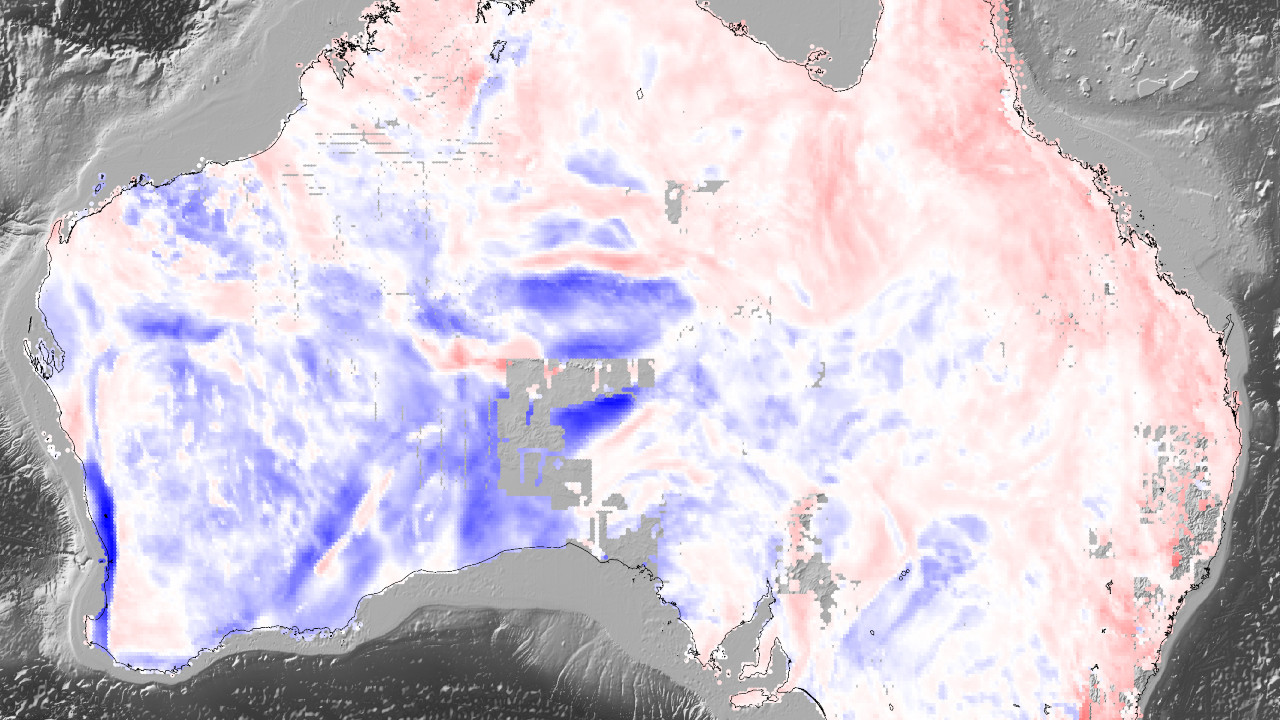
\includegraphics[width=\textwidth]{images/australia-ground-gravity-disturbance.jpg}
%  \end{center}
%  \caption{
%    Compilação de dados terrestres de distúrbio da gravidade da Austrália.
%    Distribuídos originalmente por \citet{Wynne2018}. Compilados e padronizados
%    por \citet{Uieda2021} para facilitar o seu uso em diversas linhas de
%    pesquisa.
%  }
%\end{figure}
%\begin{summarybox}[frametitle=\faInfoCircle{}\quad Resumo das atividades]
%  \begin{fa-ul}
%    \faSearchDollar & Projetos financiados pelas agências: National Science
%      Foundation (E.U.A.), Royal Society (Reino Unido) e Software Sustainability
%      Institute (Reino Unido)\\
%    \faFilePdf & 13 artigos publicados em revistas indexadas, 3 em outras
%    revistas, 11 trabalhos completos em anais de eventos\footnotemark[1] \\
%    \faComment & 38 apresentações de trabalho, sendo 13 dessas convidadas\footnotemark[1] \\
%    \aiGoogleScholarSquare & 1736 citações no \href{https://scholar.google.com/citations?user=qfmPrUEAAAAJ}{Google Scholar} e 959 no \href{https://www.webofscience.com/wos/author/record/1766625}{Web of Science} (acessados em 27/12/2022)
%  \end{fa-ul}
%\end{summarybox}
%\footnotetext[1]{O número de total trabalhos e apresentações pode ser diferente
%das quantidades listadas abaixo. Alguns trabalhos e apresentações estão
%listados em outras áreas de atuação (e.g., capítulo \ref{cap_cienciaaberta}) ou
%pertencem a mais de uma linha de pesquisa.}
%
%
%Ao longo de minha carreira, sempre busquei temas de pesquisa nos quais achava
%que meu interesse em combinar a geofísica com a programação poderia ter um
%maior impacto no avanço da ciência.
%Creio que isso se reflete no número de citações que meus trabalhos geralmente
%recebem, que é considerado alto para a área\footnote{Segundo análise da
%  plataforma Dimensions. Por exemplo
%  \url{https://badge.dimensions.ai/details/id/pub.1019631868} \citep{Uieda2012},
%  \url{https://badge.dimensions.ai/details/id/pub.1064143907} \citep{Uieda2016} e
%  \url{https://badge.dimensions.ai/details/id/pub.1059638400} \citep{Uieda2017}.
%}.
%Este capítulo é uma reflexão da minha produção científica do ponto de vista das
%diferentes linhas de pesquisa que desenvolvi, apresentadas abaixo em ordem
%cronológica com as últimas sendo as linhas mais recentemente abertas.
%
%\section{Modelagem direta de campos gravitacionais em escala global}
%\label{sec_modelagemdireta}
%
%\begin{summarybox}[frametitle=\faInfoCircle{}\quad Resumo da linha de pesquisa]
%  \begin{fa-ul}
%    \faFilePdf & 3 artigos publicados \\
%    \faFile & 1 trabalho completo em anais de eventos \\
%    \faComment & 3 apresentações de trabalho \\
%    \faUserGraduate & Alunos envolvidos: Santiago Soler (PhD), Mustafa Alordowny (BSc) \\
%    \faGlobeAmericas & País dos colaboradores: Brasil, Argentina, China, Itália, Alemanha, Canadá
%  \end{fa-ul}
%\end{summarybox}
%\begin{subsummarybox}[frametitle=\faFilePdf{}\quad Artigos publicados]
%  \begin{paperlist}
%    2019 & \Santiago, \Agustina, \Gimenez, \Me.
%      Gravitational field calculation in spherical coordinates using variable
%      densities in depth.
%      \emph{Geophysical Journal International}.
%      \DOI{10.1093/gji/ggz277}.
%      \GitHub{pinga-lab/tesseroid-variable-density}.
%      \Preprint{10.31223/osf.io/3548g}.
%      \Data{10.6084/m9.figshare.8239622}.
%      \\
%    ~ & \Guangdong, \Bo, \Me, \JLiu, \MKaban, \LChen, \RGuo.
%      Efficient 3D large-scale forward-modeling and inversion of gravitational fields in
%      spherical coordinates with application to lunar mascons.
%      \emph{Journal of Geophysical Research: Solid Earth}.
%      \DOI{10.1029/2019jb017691}.
%      \Preprint{10.31223/osf.io/dzf9j}.
%      \Data{10.6084/m9.figshare.7300523}.
%      \\
%    2016 & \Me, \Val, \Carla.
%      Tesseroids: Forward modeling gravitational fields in spherical coordinates,
%      \emph{Geophysics}, \DOI{10.1190/geo2015-0204.1}.
%      \GitHub{pinga-lab/paper-tesseroids}.
%  \end{paperlist}
%\end{subsummarybox}
%\begin{subsummarybox}[frametitle=\faFile{}\quad Trabalhos completos em anais de eventos]
%  \begin{paperlist}
%    2011 & \Me, \Everton, \Carla, \Eder.
%      Optimal forward calculation method of the Marussi tensor due to a geologic
%      structure at GOCE height,
%      \emph{Proceedings of the 4th International GOCE User Workshop}.
%      \DOI{10.6084/m9.figshare.92624}.
%      \GitHub{leouieda/goce2011}.
%  \end{paperlist}
%\end{subsummarybox}
%\begin{subsummarybox}[frametitle=\faComment{}\quad Outras apresentações]
%  \begin{paperlist}
%    2010 & \Me, \Naomi, \Carla.
%      Computation of the gravity gradient tensor due to topographic masses
%      using tesseroids,
%      \emph{AGU Meeting of the Americas},
%      Foz do Iguaçu, Brazil.
%      \DOI{10.6084/m9.figshare.156858}
%      \\
%    2008 & \Me, \Naomi.
%      Utilização de tesseróides na modelagem de dados de gradiometria
%      gravimétrica,
%      \emph{XIII Simpósio de Iniciação Científica do IAG-USP},
%      São Paulo, Brazil.
%      \DOI{10.6084/m9.figshare.4779760}
%  \end{paperlist}
%\end{subsummarybox}
%
%Esta foi minha primeira linha de pesquisa, iniciada durante meu trabalho de
%conclusão de curso de Bacharelado em Geofísica na Universidade de São Paulo
%(seção~\ref{sec_usp}).
%A motivação inicial para explorar essa linha foi o lançamento do satélite
%GOCE, que efetuou medidas dos gradientes da gravidade em uma resolução espacial
%sem precedentes.
%Seria necessária uma ferramenta computacional que pudesse modelar as medições
%que seriam feitas pelo GOCE para melhor compreender suas limitações e processar
%os dados quando estivessem disponíveis.
%Métodos numéricos para a solução das integrais de Newton do campo gravitacional
%de um prisma esférico (tesseroide) já existiam
%\citep{Heck2006,Asgharzadeh2007,WildPfeiffer2008} mas nenhum havia lidado com o
%problema da acurácia variável com a distância entre os prismas e os pontos de
%observação.
%Isso me proporcionou a chance de trazer uma perspectiva diferente para a área.
%Esta linha foi a minha introdução à pesquisa com colaborações internacionais.
%Também foi a minha primeira experiência na orientação de alunos através da
%minha coorientação do Santiago.
%
%\begin{fancyenum}{\faBullseye}{Objetivos}
%  \item Desenvolver métodos numéricos para calcular o campo gravitacional e
%    suas derivadas espaciais causados por prismas esféricos (tesseroides) de
%    maneira computacionalmente eficiente e acurada.
%  \item Utilizar os métodos desenvolvidos para modelar estruturas geológicas em
%    escala continental e global.
%  \item Disponibilizar ferramentas de software livre que implementam os métodos
%    para o uso da comunidade científica.
%\end{fancyenum}
%
%\begin{fancyenum}{\faLightbulb}{Principais contribuições}
%  \item Desenvolvimento de um algoritmo de discretização adaptativa dos
%    tesseroides capaz de garantir um nível de acurácia alto para a integração
%    numérica automaticamente \citep{Uieda2016}.
%  \item Criação e disponibilização da ferramenta de software livre Tesseroids
%    para realizar os cálculos de maneria eficiente \citep{Uieda2016}.
%  \item Desenvolvimento de um método para permitir que a densidade dos
%    tesseroides variasse radialmente de maneira genérica \citep{Soler2019}
%    para uso na determinação do embasamento de grande bacias sedimentares
%    (parte da tese de doutorado do aluno \SantiagoLink{}).
%  \item Desenvolvimento de um método para acelerar o cálculo
%    em até aproximadamente 50x em determinados casos. Este método poderia então
%    ser utilizado na inversão 3D para determinar a distribuição de densidade em
%    subsuperfície \citep[][em colaboração com pesquisadores da Central
%    South University, China, e GFZ Potsdam, Alemanha]{Zhao2019} .
%\end{fancyenum}
%
%\begin{fancyenum}{\faRocket}{Impacto da pesquisa}
%  \item O software Tesseroids é amplamente utilizado para processamento de
%    dados de gravidade em escala global, o que é evidenciado pelo alto número
%    de citações que recebe\footnote{Segundo
%    \url{https://badge.dimensions.ai/details/id/pub.1064143907}}.
%  \item O Tesseroids foi utilizado para gerar malhas regulares dos gradientes da
%    gravidade gerados a partir dos dados do satélite GOCE \citep{Bouman2016}.
%  \item Os avanços feitos no método de modelagem foram fundamentais para a
%    criação de métodos de inversão \citep{Uieda2017,Zhao2019} e métodos para
%    calcular campos magnéticos de tesseroides \citep{Baykiev2016}.
%\end{fancyenum}
%
%
%
%
%\section{Determinação da espessura crustal através de distúrbios da gravidade}
%
%\begin{summarybox}[frametitle=\faInfoCircle{}\quad Resumo da linha de pesquisa]
%  \begin{fa-ul}
%    \faFilePdf & 1 artigo publicado \\
%    \faUserGraduate & Alunos envolvidos: Aidan Hernaman \\
%    \faComment & 1 apresentação de trabalho
%  \end{fa-ul}
%\end{summarybox}
%\begin{subsummarybox}[frametitle=\faFilePdf{}\quad Artigos publicados]
%  \begin{paperlist}
%    2017 &
%      \Me, \Val.
%      Fast non-linear gravity inversion in spherical coordinates with application
%      to the South American Moho,
%      \emph{Geophysical Journal International},
%      \DOI{10.1093/gji/ggw390}.
%      \Preprint{10.31223/osf.io/9ba4m}.
%      \GitHub{pinga-lab/paper-moho-inversion-tesseroids}.
%      \Data{10.6084/m9.figshare.3987267}.
%  \end{paperlist}
%\end{subsummarybox}
%\begin{subsummarybox}[frametitle=\faInfoCircle{}\quad Apresentações]
%  \begin{paperlist}
%    2017 &
%      \Me.
%      Inverting gravity to map the Moho: A new method and the open source
%      software that made it possible,
%      \emph{Department of Geology and Geophysics, \UHM},
%      Honolulu, USA.
%      \DOI{10.6084/m9.figshare.4779766}
%  \end{paperlist}
%\end{subsummarybox}
%
%Esta linha de pesquisa busca estimar a profundidade da
%\href{https://en.wikipedia.org/wiki/Mohorovi%C4%8Di%C4%87_discontinuity}{Descontinuidade de Mohorovičić}
%(Moho) através da inversão de distúrbios da gravidade.
%Se considerarmos que a contribuição da variação de densidade na
%crosta e no manto são negligenciáveis ou foram removidas, o que observamos no
%distúrbio da gravidade corrigido da topografia é puramente o efeito da variação
%na profundidade da Moho quando comparada com um nível de referência.
%O método mais utilizado para essa estimava é o de \citet{Oldenburg1974}, que
%utiliza a transformada rápida de Fourier (FFT) para estimar o relevo de uma
%interface em uma aproximação plana da Terra.
%Esse método foi utilizado em \citet{vanderMeijde2013} para estimar a espessura
%da crosta na América do Sul.
%Métodos que são adequados pra uma aproximação esférica possuem suas limitações.
%\citet{Wieczorek1998}, que é uma generalização de \citet{Oldenburg1974} para
%harmônicos esféricos, é mais adequado para aplicações globais.
%\citet{Reguzzoni2013} é mais flexível mas requer recursos computacionais
%elevados.
%
%Para a última etapa do meu doutorado (seção~\ref{sec_doutorado}), me baseei no
%trabalho de \citet{Silva2014} para desenvolver uma inversão não-linear para
%a determinação da profundidade da Moho em uma aproximação esférica.
%Meu método aprimora a generalização do método de \citet{Bott1960} feita por
%\citet{Silva2014} introduzindo regularização de suavidade.
%Para operar em uma aproximação esférica, a modelagem direta é feita utilizando
%tesseroides (seção~\ref{sec_modelagemdireta}).
%Estimativas da profundidade da Moho provenientes de dados sismológicos são
%utilizados na inversão para determinar o contraste de densidade na Moho e o
%nível de referência.
%
%Esse trabalho se beneficiou muito da infraestrutura computacional que
%desenvolvi ao longo da minha pós-graduação.
%Os softwares Fatiando a Terra (seção~\ref{sec_fatiando}) e Tesseroids
%(seção~\ref{sec_tesseroids}) foram fundamentais para a criação do método e
%o impacto que esse trabalho teve (ver ``impacto da pesquisa'' abaixo).
%Foi com esse trabalho que realmente tive evidência de que minha dedicação à
%ciência aberta e ao uso de software livre na pesquisa
%(seção~\ref{sec_software}) não seriam prejudiciais a minha produtividade
%científica.
%
%\begin{fancyenum}{\faBullseye}{Objetivos}
%  \item Estimar a profundidade da Moho através da inversão de distúrbios da
%    gravidade em uma aproximação esférica da Terra.
%  \item Superar o custo computacional alto do procedimento de inversão
%    não-linear.
%  \item Incorporar estimativas sismológicas da profundidade da Moho na inversão.
%\end{fancyenum}
%\begin{fancyenum}{\faLightbulb}{Principais contribuições}
%  \item Desenvolvi um fluxo de processamento baseado em softwares livres que
%    está sendo utilizada pela comunidade científica.
%  \item Criei um método eficiente de inversão não-linear em uma aproximação
%    esférica capaz de incorporar estimativas sismológicas na solução.
%  \item Produzi a primeira estimativa de alta resolução da profundidade da Moho
%    para a América do Sul baseada em dados de gravidade em aproximação
%    esférica.
%\end{fancyenum}
%\begin{fancyenum}{\faRocket}{Impacto da pesquisa}
%  \item O método e o código associado ao trabalho \citet{Uieda2017}
%    possibilitaram sua aplicação direta a outras regiões \citep[e.g.,][entre
%    outros]{Chisenga2019, Sobh2020, KemgangGhomsi2021}.
%  \item O código aberto foi utilizado como base para o método de
%    \citet{Haas2020}, possivelmente acelerando seu desenvolvimento.
%  \item O trabalho \citet{Uieda2017} possui um número de citações considerado
%    alto para a área\footnote{Segundo a página
%    \url{https://badge.dimensions.ai/details/id/pub.1059638400} (acessada em
%    13/01/2023)}.
%\end{fancyenum}
%
%

==============================================================================

\chapter{Atividades de Ensino, Mentoria e Extensão}
\label{cap_ensino}

\begin{figure}[h]
  \HeroFigPad
  \begin{center}
    \includegraphics[width=\textwidth]{images/atuacao_ensino.png}
  \end{center}
  \caption{
    Foto tirada durante o curso ``Best Practices for Developing and Sustaining
    Your Open-Source Research Software'' que ministrei durante o
    \href{https://github.com/agu-ossi/2019-agu-oss}{AGU Fall Meeting de 2019}
    em São Francisco, E.U.A.
  }
\end{figure}
\begin{summarybox}[frametitle=\faChalkboardTeacher{}\quad Resumo das atividades]
  \begin{fa-ul}
    \faUserGraduate & Orientações concluídas: 11 de graduação, 1 de mestrado, 1
      coorientação de doutorado \\
    \faUser & Orientações em andamento: 1 de graduação, 1 de doutorado, 1
      coorientação de doutorado \\
    \faChalkboardTeacher & 10 disciplinas de graduação ministradas \\
    \faClock & 17 cursos de curta duração ministrados internacionalmente \\
    \faCheckSquare & Habilitação em pedagogia e técnicas de ensino aplicadas ao
      ensino superior \\
    \faLightbulb & Tópicos ensinados incluem: gravimetria, magnetometria,
    sismologia, sensoriamento remoto, métodos numéricos, programação em Python,
    métodos de campo em geofísica, introdução à geologia, problemas inversos,
    geofísica global e geodinâmica da litosfera.
  \end{fa-ul}
\end{summarybox}

As atividades de ensino e mentoria de alunos são onde encontro a maior
satisfação profissional.
Quase nenhuma outra atividade oferece a oportunidade de ter um impacto positivo
direto na vida de outras pessoas.
Minha abordagem para o ensino é muito influenciada pela minha experiência na
graduação (seção~\ref{sec_usp}) e minhas atividades de ciência aberta
(capítulo~\ref{cap_cienciaaberta}).
Utilizo a computação nas minhas aulas para empoderar os alunos com as
habilidades que necessitam para explorar conceitos e dados reais de maneira
independente.
Essa abordagem se mostrou particularmente eficaz em conjunto com uma sólida
base teórica, visualizações interativas e uma seleção de dados abertos
disponíveis para os alunos.
Este capítulo relata minhas atividades de ensino, mentoria e extensão,
incluindo minha abordagem pedagógica e meu papel na criação e ministração de
disciplinas de graduação.
Minha atuação como coordenador do curso de graduação na University of Liverpool
é discutida na seção~\ref{sec_liverpool}.

\section{Orientações}
\label{sec_orientacao}

Minha primeira experiência como mentor de um jovem cientista foi a coorientação
do aluno \SantiagoLink{} junto com o
Professor Mario E. Giménez da Universidad Nacional de San Juan, Argentina,
entre 2016 e 2022.
O primeiro contato que tive com o Santiago foi através do software
Fatiando a Terra (seção~\ref{sec_fatiando}).
Em 2015, ele começou a se voluntariar com o projeto, implementando funções
para manejar dados em malhas regulares e o cálculo de espectros de potência.
Quando ele e o Mario me convidaram para coorientar sua tese de doutorado em
2016, fiquei feliz em aceitar continuar trabalhando com ele de maneira mais
regular.
Inicialmente, a proposta era que eu fosse seu orientador principal.
Mas como essa seria minha primeira orientação e seria feita inteiramente de
forma remota, achei mais prudente começar como coorientador.
O Santiago fez excelente progresso nas linha de pesquisa em modelagem com
tesseroides (seção~\ref{sec_modelagemdireta}) e camada equivalente
(seção~\ref{sec_eql}) durante seu doutorado.
Seu envolvimento no Fatiando a Terra aumentou com o tempo. Hoje em dia ele
ocupa uma posição de liderança no projeto, estabelecendo direções para o
desenvolvimento e atuando como mentor para novos membros da comunidade.
Ele é o criador e principal desenvolvedor de duas novas componentes do
Fatiando: \href{https://www.fatiando.org/harmonica}{Harmonica} e
\href{https://www.fatiando.org/choclo/}{Choclo}.
O Santiago também foi fundamental no estabelecimento do nosso grupo de pesquisa,
o \href{https://www.compgeolab.org/}{Computer-Oriented Geoscience Lab}
(CompGeoLab).
Nossas longas conversas sobre o papel da computação na ciência,
reprodutibilidade dos resultados numéricos e formas de fazer ciência aberta
foram as maiores influências que tive para estabelecer os princípios do
CompGeoLab, codificados em nosso manual
\url{https://github.com/compgeolab/manual}.
Em 2022, o Santiago defendeu sua tese de doutorado\footnote{Disponível em
\url{https://github.com/santisoler/phd-thesis}} com sucesso e continua
colaborando com o CompGeoLab regularmente.
Vale a pena apontar que, durante esses 6 anos de orientação, eu e o Santiago
nunca nos encontramos em pessoa por conta de diversos desencontros e a pandemia
de COVID.
Aprendemos juntos como criar uma relação próxima de trabalho inteiramente
online usando uma mistura de chamadas por vídeo semanais e mensagens regulares
pela plataforma Slack.
Atualmente, o Santiago está fazendo um pós-doutorado na University of British
Columbia (UBC), Canadá, sob supervisão da Professora
\href{https://lindseyjh.ca/}{Lindsey J. Heagy}.
Seu projeto inclui trabalhar no software livre
\href{https://simpeg.xyz/}{SimPEG}, desenvolvido pelo grupo da UBC, e facilitar
interações entre o SimPEG e o Fatiando a Terra.
A experiência de trabalhar com o Santigo foi um dos maiores privilégios da
minha carreira.
Santiago é um pesquisador brilhante, um engenheiro de software excepcional
e um verdadeiro amigo.

Iniciei minha segunda experiência de orientação a nível de doutorado em 2021
com a aluna \IndiaLink{} da University of Liverpool, coorientada pelo Professor
\href{https://www.pinga-lab.org/people/oliveira-jr.html}{Vanderlei C. Oliveira Jr.}
do Observatório Nacional e pelo Professor
\href{https://www.liverpool.ac.uk/~holme/}{Richard Holme} da University of
Liverpool.
A India foi nossa aluna do curso de Bacharelado em Geofísica de Liverpool e era
uma das melhores alunas de sua turma.
Ela foi selecionada pela School of Environmental Sciences para uma posição
dupla: meio período como aluna de doutorado e meio período empregada como
\textit{Graduate Teaching Assistant}, auxiliando no ensino de disciplinas de
graduação dos cursos de geociências e geografia física.
Acho importante realçar que a seleção para a vaga foi feita inteiramente
baseada no mérito da India e não levou em consideração o projeto de doutorado
ou os orientadores.
Seu projeto de doutorado iniciou uma nova linha de pesquisa para o CompGeoLab
onde buscamos aprimorar o uso de dados de aeromagnéticos para a estimativa do
fluxo geotermal na Antártica (seção~\ref{sec_antartica}).
Através desse projeto, nos envolvemos com a organização
\href{https://www.scar.org/}{Scientific Committee on Antarctic Research}
(SCAR), especificamente no grupo
\href{https://www.scar-instant.org/index.php/research-themes/theme-2-solid-earth-ice-interactions/sc1-antarctic-geothermal-heat-flux}{SC1
Antarctic Geothermal Heat Flux}.
A India também estabeleceu contato com pesquisadores da British Antarctic
Survey, que criaram a compilação de dados magnéticos antárticos ADMAP2
\citep{Golynsky2018}, para obter os dados brutos e consultá-los sobre os
detalhes do processamento que fizeram.
A India é uma pesquisadora com atitude excepcionalmente profissional e
com iniciativa própria, além de ser dedicada e inteligente.
Seu projeto ainda está em fase inicial mas tenho certeza de que ela produzirá
trabalhos excelentes.

Também em 2021, fui convidado pelo Professor Ricardo I. F. Trindade a
coorientar o aluno de doutorado \GelsonLink{} da Universidade de São Paulo.
Eu e o Ricardo havíamos conversado durante encontros no AGU Fall Meeting sobre
algumas ideias de adaptar técnicas de métodos potenciais, como a deconvolução
de Euler (seção~\ref{sec_euler}), a dados de microscopia magnética.
O Gelson se juntou ao CompGeoLab para dar início a essa nova linha de pesquisa
(seção~\ref{sec_micromag}), me trazendo de volta ao assunto da minha primeira
iniciação científica na USP (seção~\ref{sec_usp}).
Em apenas um ano, o Gelson já foi bem sucedido na adaptação da deconvolução de
Euler e o método de \citet{OliveiraJr2015}, junto com técnicas de processamento
de imagens que aprendi com minha disciplina de sensoriamento remoto em
Liverpool (seção~\ref{sec_ensino_grad}), para estimar o momento de dipolo
de grãos individuais de minerais ferromagnéticos.
Em 2022, fomos contemplados com um projeto da
\href{https://royalsociety.org/}{Royal Society} para realizar intercâmbios
entre a São Paulo e Liverpool para dar início à colaboração entre as duas
instituições.
Até o momento, utilizamos o financiamento da Royal Society para trazer o Gelson
para Liverpool e trabalharmos em seu primeiro artigo, que está nos processos
finais de escrita antes da submissão.
Orientar o Gelson tem sido um verdadeiro privilégio.
Ele é respeitoso, dedicado, inteligente, possui uma base sólida em geociências,
tem iniciativa própria e aprende rapidamente conceitos novos que estão fora de
sua zona de conforto.
Não tenho dúvida de que nossa colaboração produzirá pesquisa de alto impacto
nessa linha emergente.

Fui o orientador de 11 trabalhos de conclusão de curso e uma dissertação de
mestrado do curso de geofísica da University of Liverpool, com alunos
atuando em diversas linhas de pesquisa\footnote{Uma lista completa dos alunos
e seus projetos está disponível no meu Currículo Lattes: \url{https://lattes.cnpq.br/\Lattes}}.
Aprendi com essas orientações como guiar alunos sem experiência prévia em
pesquisa pelas etapas iniciais de um projeto e como ajustar o nível dos
projetos propostos com o nível dos alunos no final de um curso de graduação no
Reino Unido.
Foi particularmente gratificante observar os alunos progredirem durante seus
projetos e produzirem trabalhos de conclusão com uma qualidade muito acima do
que eles achavam que seriam capazes.


\section{Cursos de curta duração}
\label{sec_workshops}

\begin{subsummarybox}[frametitle=\faClock{}\quad Cursos e workshops ministrados online]
  \begin{paperlist}
    2022 &
      Crafting beautiful maps with PyGMT.
      \textit{EGU General Assembly}.
      \GitHub{GenericMappingTools/egu22pygmt}
      \\
    ~ &
      A geophysical tour of mid-ocean ridges.
      \textit{Transform 2022} (online).
      \GitHub{leouieda/transform2022}.
      \YouTube{NzJmRlJCNbQ}
      \\
    2021 &
      The Generic Mapping Tools for Geodesy.
      \textit{UNAVCO} (online).
      \GitHub{GenericMappingTools/2021-unavco-course}
      \\
    2020 &
      Let's build a geophysical inversion with Python.
      \textit{IRTG-2379 Graduate School: Modern Inverse Problems},
      \textit{RWTH Aachen University} (online).
      \GitHub{compgeolab/2020-aachen-inverse-problems}
      \\
    ~ &
      The Generic Mapping Tools for Geodesy.
      \textit{UNAVCO} (online).
      \GitHub{GenericMappingTools/2020-unavco-course}.
      \YouTube{EQgxDmCXvj4}
      \\
    ~  &
      From scattered data to gridded products using Verde.
      \textit{Transform 2020} (online).
      \GitHub{fatiando/transform2020}.
      \YouTube{-xZdNdvzm3E}
  \end{paperlist}
\end{subsummarybox}
\begin{subsummarybox}[frametitle=\faClock{}\quad Cursos e workshops ministrados presencialmente]
  \begin{paperlist}
    2019 &
      Best Practices for Developing and Sustaining Your Open-Source Research Software.
      \textit{AGU Fall Meeting}.
      \GitHub{agu-ossi/2019-agu-oss}
      \\
    ~  &
      Become a Generic Mapping Tools Contributor Even If You Can't Code.
      \textit{AGU Fall Meeting}
      \\
    ~  &
      The Generic Mapping Tools for Geodesy.
      \textit{Scripps Institution of Oceanography} and \textit{UNAVCO}.
      \GitHub{GenericMappingTools/2019-unavco-course}.
      \YouTube{uPUt4\_kd6m8}
      \\
    ~  &
      Introduction to Python Workshop (Earth Sciences REU program).
      \textit{Department of Geology and Geophysics, \UHM}.
      \GitHub{leouieda/2019-06-reu-python}
      \\
    2018 &
      Best Practices for Modern Open-Source Research Codes.
      \textit{AGU Fall Meeting}.
      \GitHub{agu-ossi/2018-agu-oss}
      \\
    ~  &
      Git and GitHub: What are their uses? Are they worth the effort? Let's find out!
      \textit{ASPRS UHM Student Chapter, \UHM}
      \\
    2017 &
      Introduction to Python.
      \textit{Department of Geology and Geophysics, \UHM}.
      \GitHub{leouieda/python-hawaii-2017}
      \\
    2016 &
      Python for Geologists (SAGEO).
      \textit{Faculdade de Geologia, \UERJ}.
      \GitHub{leouieda/python-geologia-2016}
      \\
    ~  &
      Python como uma ferramenta numérica em Ciências da Terra: uma nova
      abordagem de programação.
      \textit{XVIII Escola de Verão de Geofísica do IAG-USP}.
      \GitHub{leouieda/verao2016}
      \\
    2014 &
      Tópicos de inversão em geofísica.
      \textit{III Semana de Geofísica da UnB}.
      \GitHub{pinga-lab/inversao-unb-2014}
      \\
    2012 &
      Tópicos de inversão em geofísica.
      \textit{XVI Escola de Verão de Geofísica do IAG-USP}.
      \GitHub{pinga-lab/inversao-iag-2012}
  \end{paperlist}
\end{subsummarybox}

Minha primeira experiência com o ensino foi através do curso ``Tópicos de
inversão em geofísica'' que ministrei em 2012 junto com meu amigo e então
colega de doutorado
\href{https://www.pinga-lab.org/people/oliveira-jr.html}{Vanderlei C. Oliveira Jr.}
na XVI Escola de Verão de Geofísica do IAG-USP.
Foi durante esse curso que percebi minha paixão pelo ensino e decidi seguir a
carreira acadêmica para poder combinar ensino, pesquisa e extensão.
Desde então, ministrei diversos cursos de curta duração e workshops em formato
online e presencial.
Esses cursos complementam o ensino tradicional em disciplinas de graduação e
pós-graduação, fornecendo a oportunidade de experimentar com tecnologias,
formatos de ensino e tópicos pouco tradicionais.

A maioria dos cursos que ministrei estão relacionados à programação. O formato
curto é adequado para uma introdução à conceitos básicos de programação ou
para abordar um assunto específico (e.g., como criar mapas com o
\href{https://www.pygmt.org}{PyGMT},
como interpolar dados com o \href{https://www.fatiando.org/verde}{Verde}
ou como criar testes unitários para seu software).
Por isso, acho as ``escolas de verão'' e ``semanas da geofísica'' organizadas
pelas universidades tão proveitosas.
Esses cursos também podem fornecer aos alunos um contato com especialistas de
todo o mundo.
Esse contato pode inclusive ser feito com um orçamento limitado
devido aos avanços recentes nas plataformas de vídeo conferência e a difusão de
atividades online causados pela pandemia de COVID.


\section{Disciplinas de graduação}
\label{sec_ensino_grad}

\begin{subsummarybox}[frametitle=\faGraduationCap{}\quad Disciplinas ministradas na \UERJ{}]
  \begin{courselist}
    2015--2016 &
      IME03-1366 Matemática Especial I.
      \newline
      \GitHub{mat-esp/about}
      \\
    2014--2016 &
      FGEL04-12422 Geofísica II.
      \newline
      \GitHub{leouieda/geofisica2}
      \\
    ~ &
      FGEL04-12421 Geofísica I.
      \newline
      \GitHub{leouieda/geofisica1}
      \\
    2015 &
      FGEL01-00805 Geologia Geral I.
  \end{courselist}
\end{subsummarybox}
\begin{subsummarybox}[frametitle=\faGraduationCap{}\quad Disciplinas ministradas na University of Liverpool]
  \begin{courselist}
    2023--atual  &
      ENVS219: Earth and Environmental Data Science (\textit{em
      desenvolvimento}).
      \\
    2020--atual  &
      ENVS398: Global Geophysics and Geodynamics.
      \newline
      \GitHub{leouieda/lithosphere}
      \\
    ~ &
    ENVS258: Environmental Geophysics.
      \newline
      \GitHub{leouieda/remote-sensing}.
      \newline
      \GitHub{leouieda/gravity-processing}.
      \\
    ~ &
    ENVS386: Geophysical Data Modelling.
      \newline
      \GitHub{leouieda/ml-intro}.
      \\
    ~ &
      ENVS101/106: Study Skills and GIS (tutorial).
      \\
    2019--2021 &
      ENVS123: Introduction to Geoscience and Earth History.
      \\
    2019--2020  &
      ENVS362: Geophysics Field School.
  \end{courselist}
\end{subsummarybox}

Na \UERJ{}, tive a oportunidade de criar o conteúdo de três disciplinas de
graduação: Matemática Especial I e Geofísica I e II.
A disciplina Matemática Especial I pertence ao curso de Bacharelado em
Oceanografia e cobria tópicos avançados de matemática.
Meu papel ao assumir essa disciplina era convertê-la em uma introdução à
programação em Python e ao cálculo numérico.
Decidi incluir no início da disciplina uma introdução ao software de controle
de versão \href{https://git-scm.com/}{git} e à plataforma
\href{https://github.com/}{GitHub}.
Assim, pude manejar a disciplina inteiramente pelo GitHub, com cada lição
sendo armazenada em um repositório da organização
\url{https://github.com/mat-esp}.
Durante as aulas práticas, os alunos se dividiam em grupos e cada grupo era
automaticamente fornecido com uma cópia do repositório da lição pela plataforma
\href{https://classroom.github.com/}{GitHub Classroom}.
Ao final da aula, os alunos submetiam suas soluções para a tarefa da lição
também pelo GitHub, onde recebiam as notas e correções.

As disciplinas de geofísica, cobrindo uma introdução aos métodos geofísicos,
são parte do curso de Bacharelado em Geologia e haviam acabado de serem
reformuladas quando assumi meu cargo na UERJ em 2014.
Logo, pude criar o conteúdo das disciplinas por conta própria e estabelecer
como gostaria que fossem estruturadas.
Optei por dividi-las entre aulas teóricas e aulas práticas computacionais.
Nas práticas, utilizei o software \href{https://jupyter.org/}{Jupyter} para
criar \textit{notebooks} que explicavam os conceitos abordados em aula
utilizando uma combinação de texto, equações, código pronto para demonstrar os
conceitos, tarefas para serem executadas através de visualizações interativas
(figura~\ref{fig_notebooksismica}) e perguntas para serem respondidas como
parte da avaliação somativa da disciplina.
Essa abordagem foi bem recebida pelos alunos.
Inclusive, fui escolhido como paraninfo da turma de formandos da Geologia em
2016 (ano de ingresso 2012).

\begin{figure}[t]
  \begin{center}
    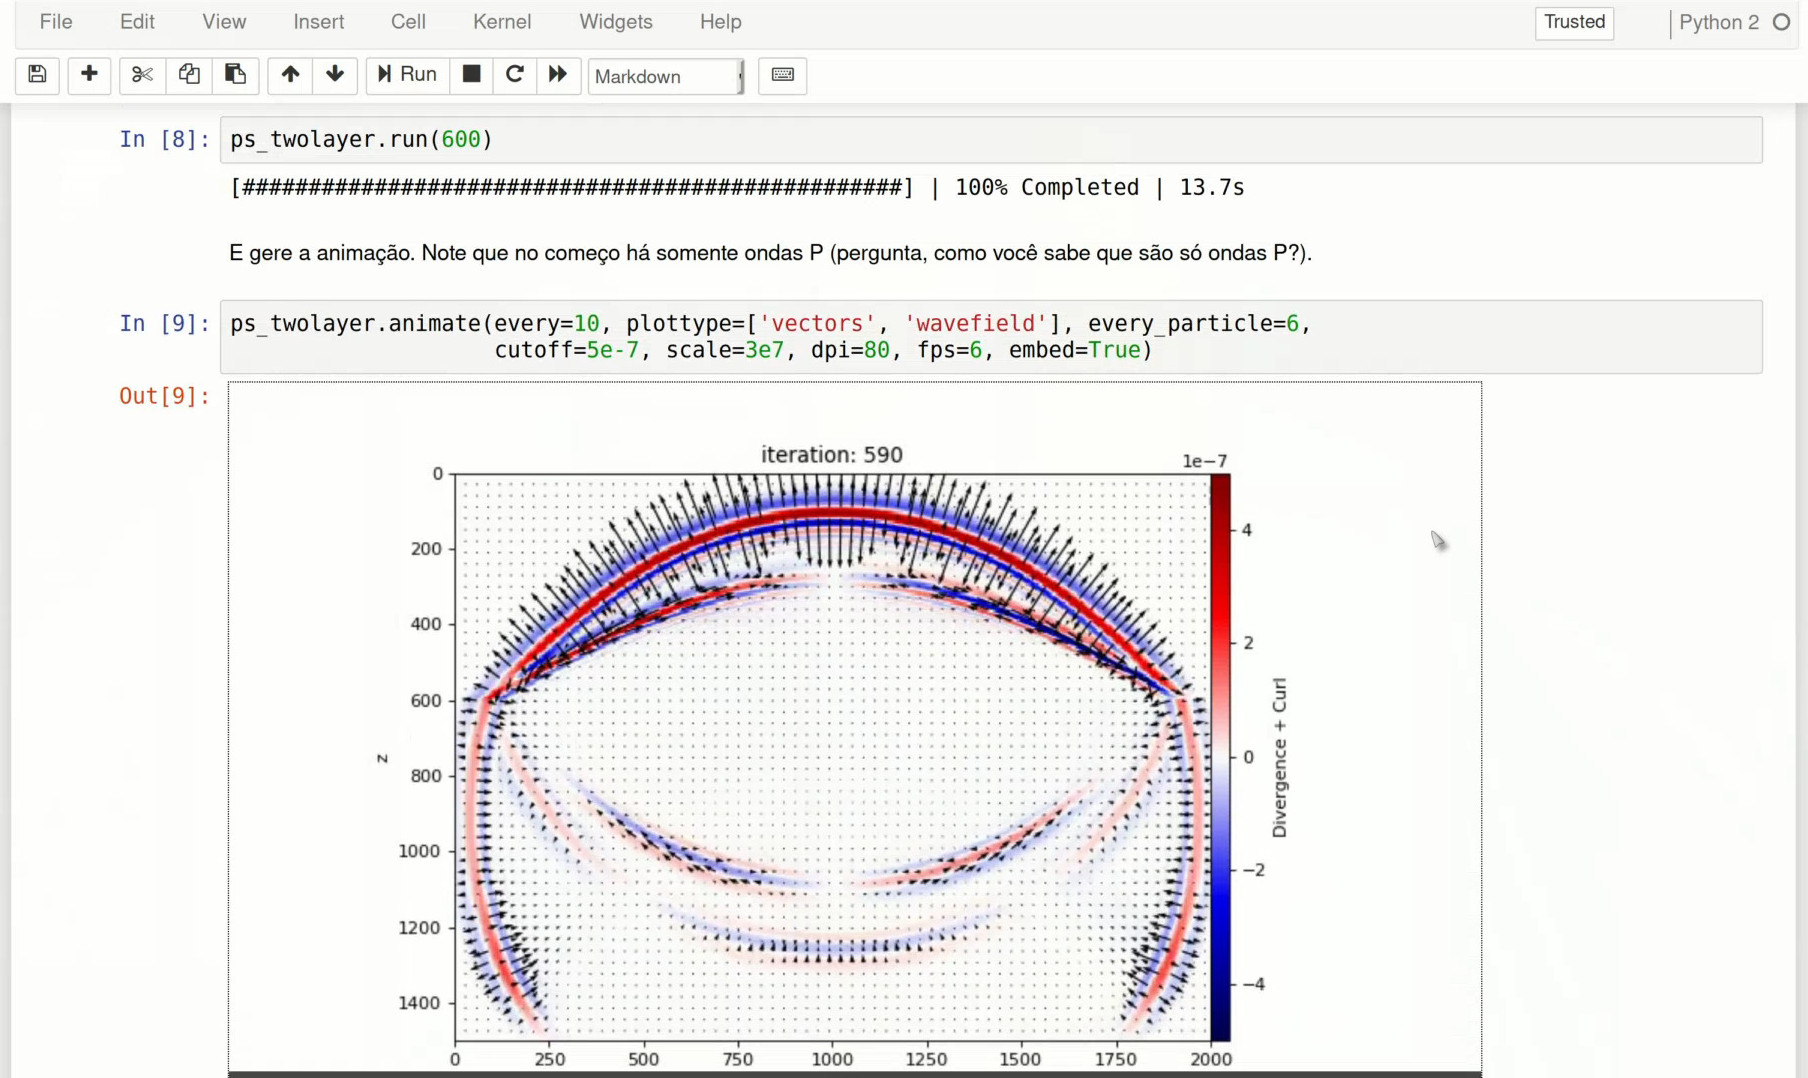
\includegraphics[width=\textwidth]{images/seismic-waves-demo.jpg}
  \end{center}
  \caption{
    Exemplo de um notebook usado na minha disciplina ``Geofísica 2'' da UERJ
    para ensinar o conceito de ondas sísmicas, reflexão, refração e conversão
    de ondas P em ondas S ao interagir com uma interface geológica. O notebook
    contém instruções, teoria, perguntas e código pronto que os alunos
    podem executar e modificar para criar animações da propagação de ondas
    elásticas (utilizando o código de diferenças finitas do Fatiando a Terra).
    A figura no notebook é parte de uma animação da propagação de uma onda P
    que incide sobre uma interface, gerando ondas P e S refletidas e
    refratadas.
    As cores representam a soma do divergente e o rotacional do campo de
    deformações, mostrando as frentes de onda.
    Vetores indicam o deslocamento de cada ponto do modelo, com ondas P e S
    tendo deslocamento perpendicular e paralelo às frentes de onda,
    respectivamente.
  }
  \label{fig_notebooksismica}
\end{figure}

Na University of Liverpool, participei de diversas disciplinas dos cursos de
Geofísica e Geologia, ministrando
programação em Python para Ciências da Terra em ``ENVS101
Study Skills and GIS'',
introdução à estrutura da Terra e isostasia em ``ENVS123 Introduction to
Geoscience and Earth History'',
inversão não-linear e aprendizagem de máquinas em ``ENVS386 Geophysical Data
Modelling''
e a matéria de campo do terceiro ano de geofísica
``ENVS362 Geophysics Field School''.
Continuo com a abordagem computacional que desenvolvi na UERJ, dessa vez
incluindo tarefas onde os alunos devem escrever parte do código.
Atualmente, adotei a metodologia de
\href{https://pt.wikipedia.org/wiki/Aula_invertida}{aula invertida}, produzindo
vídeos explicando a base teórica para os alunos assistirem independentemente e
utilizando todo o tempo em sala de aula para atividades práticas com os
notebooks e discussões.

Criei a nova disciplina optativa ``ENVS398: Global Geophysics and Geodynamics''
junto com o Professor
\href{https://www.liverpool.ac.uk/environmental-sciences/staff/andrew-biggin/}{Andy Biggin}.
Utilizamos aulas gravadas para ensinar o conteúdo teórico.
As partes práticas da disciplina são dividas em duas partes.
Durante metade da disciplina, ministrada pelo Andy, os alunos aprendem sobre o
núcleo e o manto terrestre, discutindo artigos recentes da literatura durante
as aulas presenciais.
Durante a outra metade da disciplina, ministrada por mim, os alunos aprendem
sobre a geodinâmica da litosfera.
Nas aulas práticas, os alunos desenvolvem a implementação computacional dos
modelos abordados nas aulas teóricas e os comparam a dados reais.
Utilizo os notebooks com parte do seu código fornecido por mim para os alunos
construírem suas soluções em etapas gradativamente mais desafiadoras.
Também utilizo um conjunto global de dados de distúrbios da gravidade, fluxo de
calor geotermal, topografia e idade do assoalho oceânico para os alunos
interpretarem e processarem livremente.
Essa matéria foi consistentemente elogiada pelos alunos nos formulários de
avaliação semestrais das disciplinas.

Sou o responsável pela disciplina ``ENVS258 Environmental Geophysics'' onde
ensino uma introdução ao sensoriamento remoto, processamento e aquisição de
dados de gravidade e com uma componente de campo, onde introduzimos aos alunos
os equipamentos que possuímos em Liverpool (magnetometria, GRP,
eletrorresistividade, GPS, EM-31 e refração sísmica).
Desenvolvi todo o material prático para a componente de sensoriamento remoto,
utilizando novamente os notebooks e dados abertos dos satélites Landsat
fornecidos na plataforma \href{https://earthexplorer.usgs.gov/}{EarthExplorer}
da USGS.
A avaliação somativa dessa componente é um relatório onde os alunos escolhem um
tema dentro do escopo da disciplina, fazem a pesquisa bibliográfica, baixam os
dados relevantes do EarthExplorer, processam os dados usando notebooks em
Python e geram suas visualizações e conclusões.
Para a grande maioria dos alunos, essa é sua primeira tarefa independente e o
seu primeiro contato com a pesquisa.
A qualidade e criatividade dos relatórios que os alunos produzem frequentemente
me surpreende.
Em múltiplas ocasiões, incorporei o trabalho de alunos nas minhas aulas porque
eram simplesmente superiores aos exemplos que eu pude desenvolver\footnote{Por
exemplo, as práticas
\url{https://github.com/leouieda/remote-sensing/blob/main/practicals/practical2.ipynb}
e
\url{https://github.com/leouieda/remote-sensing/blob/main/practicals/practical4.ipynb}}.
A componente de sensoriamento remoto é sempre elogiada pelos alunos nas
avaliações do curso, o que me dá muito orgulho porque foi um tema que aprendi
quase inteiramente através de ministrar essa disciplina.

Estou criando a disciplina ``ENVS229 Earth and Environmental Data Science'' com
os Professores \href{https://www.liverpool.ac.uk/environmental-sciences/staff/ben-edwards/}{Ben Edwards}
e \href{https://www.liverpool.ac.uk/environmental-sciences/staff/greig-paterson/}{Greig Paterson}.
Essa disciplina fornecerá conhecimentos intermediários de programação em Python
e técnicas de estatística e análise de dados geocientíficos para todos os
cursos de Ciências da Terra do departamento.
Isso é atualmente possível porque em 2021 introduzi um curso de programação em
Python na disciplina do primeiro ano ``ENVS101 Study Skills and GIS'',
fornecendo aos alunos a base necessária para cursar a nova disciplina.
Nosso desejo de criar essa disciplina foi motivado pela falta de treinamento
que os nossos alunos de geologia e geografia física recebem em análise de
dados, atividade que atualmente é altamente valorizada por empregadores em
geociências e ciência de dados.

\section{Atividades de Extensão}

Minhas atividades na área de extensão universitária são mais limitadas que
minha atuação em outras áreas.
Parte da razão é meu foco adicional em outras atividades, como minha atuação
em ciência aberta (capítulo~\ref{cap_cienciaaberta}).
Por conta da pandemia de COVID de 2020, muitas das atividades de extensão que
eram promovidas pela universidade estavam canceladas durante a maior parte da
minha estadia em Liverpool.
Em 2022, com a retomada das atividades presenciais, participei de três eventos
na University of Liverpool chamados de \textit{Open Days}, durante os quais
os alunos de ensino médio visitam a universidade para conhecer mais sobre os
cursos oferecidos.
Na parte das Ciências da Terra, fizemos demonstrações sobre como a viscosidade
influencia o fluxo de lava, como o Ground Penetrating Radar (GPR) detecta
objetos em subsuperfície e como o conceito de isostasia explica a espessura
crustal em regiões montanhosas.
Além dos Open Days, fui voluntário no evento \textit{Hour of Code} para ensinar
programação para alunos de ensino fundamental da Salt Lake Elementary School em
Honolulu, E.U.A.
Também fui entrevistado nos podcasts de divulgação das geociências
\href{https://undersampledrad.io}{Undersampled Radio}
(episódio ``\href{https://undersampledrad.io/home/2016/7/open-sourcery}{Open
Sourcery}'' de 19/05/2016)
e \href{https://www.dontpanicgeocast.com/166}{Don't Panic Geocast}
(episódio ``\href{https://www.dontpanicgeocast.com/166}{You are headed to a warm and sunny place}''
de 27/04/2018).
Essas atividades são extremamente gratificantes e gostaria de dedicar mais
tempo a elas no futuro.
Em particular, gostaria de expandir uma atividade que desenvolvi para explicar
aquisições aeromagnéticas utilizando ímãs enterrados e o aplicativo de celular
\href{https://phyphox.org/}{Phyphox}, que dá acesso aos dados registrados pelos
magnetômetros dos celulares modernos.


==============================================================================

\chapter{Conclusão}
\label{cap_conclusao}

Este memorial contém um relato dos últimos 19 anos, desde minha entrada no
curso de Bacharelado em Geofísica da Universidade de São Paulo até minha
posição atual como Lecturer na University of Liverpool.
Ao longo desse caminho, passei por 6 instituições em 4 países, fui autor de 16
artigos científicos e 10 softwares livres para ciência, ministrei 10
disciplinas diferentes de graduação e orientei e coorientei 16 alunos de
graduação, mestrado e doutorado.
Atuo em diversas linhas de pesquisa relacionadas a problemas inversos em
métodos potenciais, com aplicação na prospecção de recursos naturais e estudos
da crosta terrestre em escala continental.
Tenho uma forte convicção de que a ciência deve ser feita de forma
transparente, reprodutível, reutilizável e cooperativa.
Por isso, invisto uma grande parte do meu tempo e esforço em iniciativas que
apoiam a ciência aberta e o uso de software livre na ciência e na educação.
O ensino e a interação com os alunos são meus maiores motivadores
profissionais.
Não consigo me imaginar atualmente em uma carreira na qual não tenho a
oportunidade de ser professor e mentor.

Embora minha experiência em Liverpool tenha sido gratificante e possibilitado
meu crescimento profissional, descobri alguns aspectos da academia na
Inglaterra que a tornam menos atrativa para mim.
Por exemplo, a natureza extremamente comercial do ensino superior, a grande
disparidade de salários e o curso extremamente curto de Bacharelado de apenas
aproximadamente 50 dias de aulas por semestre ao longo de três anos (comparado
com aproximadamente 100 dias por semestre ao longo de quatro ou cinco anos nas
universidades brasileiras).
Este último fator resulta em alunos entrando na pós-graduação com menos
preparo, o que significa que projetos que eu julgaria a nível de doutorado no
Brasil são a nível de pós-doutorado para alunos do Reino Unido.
Também tive minha filha Yara em 2020 e, por conta das restrições em viagens
internacionais, não tive suporte familiar algum.
Percebo agora mais do que nunca o quanto a proximidade da família contribui
para o bem-estar e o balanço saudável entre o trabalho e a vida pessoal.
A longo prazo, todos esses fatores podem no futuro resultar em uma produção
científica e pedagógica que está abaixo das minhas perspectivas profissionais.

As circunstâncias familiares e profissionais que tenho agora são muito
diferentes do que eram cinco anos atrás quando decidi sair do meu emprego na
UERJ.
Aprendi muito com os últimos seis anos que passei em instituições
internacionais.
Pude estabelecer relações duradouras com pesquisadores excelentes e
experienciar como diferentes culturas abordam o ensino superior e o
financiamento para pesquisa.
Desde minha primeira experiência no exterior na York University
(seção~\ref{sec_york}), aprecio cada vez mais o que temos no Brasil e, em
particular, na Universidade de São Paulo.
Obter os títulos de Bacharel, Mestre e Doutor sem acumular uma dívida
gigantesca é um privilégio que poucos tem nos E.U.A., Canadá e Inglaterra.
Devo muito ao país que me providenciou um ensino superior de qualidade
excepcional de forma gratuita e bolsas para realizar a pós-graduação.
Sinto que agora está na hora de retribuir meu país com a experiência que
adquiri no Brasil e no exterior em pesquisa, ensino, administração e extensão.

Caso tenha a oportunidade, pretendo buscar colaborações com os pesquisadores e
pesquisadoras do IAG e do IGc nas áreas de estrutura crustal da América do Sul,
de aplicações geoambientais (e.g., através do sensoriamento remoto), de
gravimetria e geodésia física, de desenvolvimento de software (e.g., através
dos aplicativos do grupo de sismologia e do envolvimento tradicional do IAG no
Generic Mapping Tools) e de paleomagnetismo.
Adoraria ter a chance de expandir minha atuação na extensão universitária,
especialmente na divulgação da geofísica através de visitas a escolas, nos
cursos de Geofísica para a Terceira Idade do IAG e na produção de recursos
educacionais abertos em português.
Também vejo que posso contribuir em diversos aspectos dos cursos de graduação
e pós-graduação.
Uma mudança no curso desde minha passagem pela USP que me chamou a atenção foi
a introdução das disciplinas ``Problemas Integrados em Ciência da Terra I e
II''.
Essas disciplinas visam fornecer uma ponte entre o ciclo básico e o conteúdo de
geofísica, um aspecto do qual sentia falta durante meu curso de graduação.
Os tópicos cobertos por essas disciplinas possibilitam o uso das técnicas
computacionais de ensino que utilizo em minhas aulas.
Possuo experiência prévia de ensino nos tópicos das disciplinas do concurso:
métodos potenciais, geofísica e geodinâmica global, estrutura interna da Terra
e sismologia.
Além das disciplinas especificadas no concurso, eu teria a capacidade de
propor disciplinas optativas e de pós-graduação nos tópicos de gravimetria,
engenharia de software científico (complementando a disciplina AGG0204),
métodos quantitativos de sensoriamento remoto, aprendizagem de máquina aplicada
a Ciência da Terra, entre outros.
Continuaria a oferecer cursos de curta duração presenciais e online,
particularmente os cursos da organização
\href{https://softwareunderground.org/}{Software Carpentry} da qual sou um
instrutor credenciado.
Gostaria também de propor o uso da observação por pares como uma técnica para
difundir boas práticas pedagógicas, porque acredito ter coisas a
contribuir assim como sei que tenho muito a aprender.
Em suma, seria uma honra ter a chance de fazer minha parte para formar os
alunos brasileiros e contribuir para a Universidade de São Paulo.


%==============================================================================
\backmatter
\bibliographystyle{apalike-doi}
\bibliography{references}

\end{document}
